\documentclass[a4paper,12pt]{report}

\usepackage[]{geometry} %textwidth=6.5in,textheight=9in
\usepackage{graphicx}
\usepackage{graphics}
\usepackage{amsmath}
\usepackage{url}
\usepackage{float}
\usepackage{hyperref}
\usepackage{listings}
\usepackage{minted}
\usepackage{pdflscape}
\usepackage{rotating}
\usepackage{mdframed}

\hypersetup{ colorlinks=true, linkcolor=blue, filecolor=magenta, urlcolor=cyan }
\renewcommand\listoflistingscaption{List of source codes}

\begin{document}

\begin{titlepage}
	\begin{center}
		%\vspace*{1cm}
		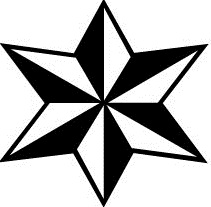
\includegraphics[scale=1,width=0.3\textwidth]{images/uob_logo} \\
		\huge
		\textbf{Machine Learning in Drug Discovery and Design\\}
		\vspace{0.5cm}
		\Large
		Predicting the Blood Brain Barrier Penetration of Drugs \\
		\vspace{1.5cm}
		\textbf{Ibraheem Ajibola Ganiyu}
		\vfill
		A dissertation presented for the degree of \\
		BSc. (Hons) Software Engineering. \\
		\vspace{0.8cm}
		\large
		School of Computing, Engineering and Mathematics \\
		University of Brighton \\
		\date{\today}
	\end{center}
\end{titlepage}

\pagenumbering{roman}
\tableofcontents
\newpage
\listoffigures
\listoftables
\listoflistings
\newpage
\pagenumbering{arabic}


\begin{abstract}
	Drug design and discovery is a very expensive process and lots of new compounds are being developed rapidly. Only roughly about 2\% of drugs can pass through the blood brain barrier, this presents a problem in Central Nervous System (CNS) drug development. \\
	This Project aims to develop a solution that can predict with high confidence, the probability of a drug passing through this blood brain barrier in hopes that this can speed up the process of developing a CNS drug.
\end{abstract}

\chapter{Introduction}
	Chemical data is growing exponentially as there are currently more than 123 million organic and inorganic substances to date \cite{CAS2016}, which means for drug development purposes, there is an abundance of chemical data to analyse in search for ideal candidates for development. \\
	Machine Learning is a form of artificial intelligence (AI) that enables computer programs to learn concepts from data without being explicitly programmed. This technique of AI can be applied to problems in many domains, which is what this paper aims to do by applying it to chemical data to build computer models, aka Virtual Screening, models which can predict with high accuracy, the probability of a drug to pass through the blood brain barrier (BBB) of living organisms. \\
	\textit{In Silico} models (computer models) have a profound use in virtual screening as they can enable scientist to scan through a large database of drugs to speed up a time consuming process of analysing drug candidates. \\
	In the context of CNS (Central Nervous System) drug development, when a drug is absorbed into the blood stream, it needs to be able to pass through the Blood Brain Barrier (BBB) to its target which could be the brain or the nervous system, an example would an anti-migraine agent, ergotamine, 
		\begin{figure}[H]
			\centering
			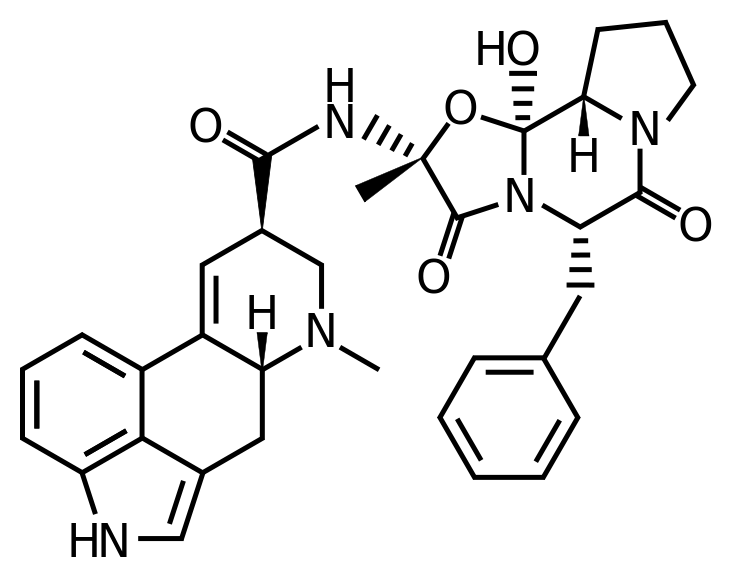
\includegraphics[scale=1,width=0.55\textwidth,totalheight=0.3\textheight]{images/Ergotamine-skeletal} 
			\caption{Chemical Representation of Ergotamine}
			\label{fig:ergotamine}
		\end{figure}
	which has to pass through the blood brain barrier to the lining of the brain where it constricts the blood vessels there to decrease the pain from migraine headaches \cite{DrugsCom}. 
	%TODO: This needs citation -> 2% of known molecules
	However statistically speaking, only 2\% of the currently known molecules can pass through this blood brain barrier, which translates to more time in the drug discovery pipeline spent on analysing drug candidates that can pass through the BBB barrier. \\
	\section{Proposed Solution}
		This problem of determining the drug candidates that belong to this 2\% is a very challenging one and this paper approaches the problem through the use of computer models built with machine learning techniques, applied to a large database of molecules that pass through the Blood Brain Barrier, with the aim of predicting the probability of an unknown candidate drug passing through the BBB. \\
		Ana et al \cite{Anaetal2012} points out that there is a lack of extensive dataset on BBB prediction as most of them are not comprehensive enough to build complex models out of, as a result, they have compiled a dataset of 2040 molecules for use in BBB prediction. Based on analysis carried out \cite{Anaetal2012} by Ana et al, They show that certain machine learning classifiers such as support vector machines and random forests outperform other classifiers especially for BBB classification tasks. This paper will attempt utilise that analysis as a baseline for developing our computer models whilst also exploring the possibility of Deep neural networks, as Thomas et al \cite{Thomasetal2014} show that Deep learning techniques have a significant opportunity in virtual screening.
	\section{Results}


\chapter{Background}
	Everything around us is composed of molecules, they are an electrically neutral group of two or more atoms held together by chemical bonds. They are the smallest particle in a compound that exhibit the chemical properties of the compound. 
	Trees can be said to be made up of molecules and historically parts of trees have always been used to cure or alleviate symptoms of illness. Over time, the individual molecules in these herbal medicines were recognized for their effects and they were being produced synthetically, which further gave rise to Modern Drug Design and Discovery. \\
	A potential molecule aka drug candidate is usually screened against a target protein to test its effectiveness and the screening can either be virtual (Virtual Screening) or through a method known as High Throughput Screening (HTS) - a method of experimentation involving the use of robots and control software to conduct millions of scientific tests. These HTS machines can also be credited with the exponential growth in chemical data \cite{Dougetal2008}.
	Drug discovery is a very expensive and time consuming process; It is usually broken down into numerous stages with the most expensive stage being the clinical trials. \\
	The problem of the Blood Brain Barrier (BBB) prediction evolves around Chemistry and Computer Science being applied to the Drug Design domain with a thorough understanding of the constrainsts imposed by the Central Nervous System. This chapter introduces the necessary concepts needed to understand the solution taken to the BBB prediction problem.
	
	
	\section{Cheminformatics}
	Cheminformatics also known as Chemoinformatics or Chemical Informatics can be visualised as a cross domain of Chemistry and Computer Science. As defined by Brown, it is the mixing of numerous information that a scientist needs to transform data into information for the intended purpose of making better decisions in drug lead identification and optimisation \cite{FKBrown1998}. \\
	The applications of Cheminformatics that are of particular interest are \textit{Storage and Retrieval of Chemical Data} and \textit{Virtual Libraries and Screening} as they both would enable the manipulation and transformation of molecular information for our machine learning algorithms. 
		\subsection{Representing Molecules in Computers}
		The two most common formats for representing chemical molecules in computers are Simplified Molecular-Input Line Entry System (SMILES) and SMART, with SMART being created by Daylight Chemical Information Systems and both formats being actively supported by them \cite{OpenBabel2017}.
			\paragraph{SMILES} are specifications in the typographical notation system that describe the structure of a molecule using short ASCII strings and they are more commonly used. Water can be written in the SMILE format as $[OH2]$ An example would be the SMILE representation of protriptyline
				\begin{equation*}
					CNCCCC1c2ccccc2C=Cc3ccccc13
				\end{equation*}
			This format can then be utilised by cheminformatics software to extract meaningful chemical information about the molecule. Throughout the project, the Open-Source Cheminformatics Software, \href{www.rdkit.org}{RDKit}, was used to transform the SMILEs in the dataset and also for the extraction of molecular information, which will be explained below.
		\subsection{Molecular Representation and Similarity}
		Similar molecules exhibit similar properties \cite{JohnMaggiora1990}, with this knowledge, it is possible to approach the BBB problem with the idea that if we know for a given molecule $x$, that it can pass through the Blood Brain Barrier, then we can expect another given molecule $y$ which is similar to $x$ to pass through the barrier. \\
		This further raises the question of how to represent a molecule (Molecular Representation) in a format that can enable us to compare its similarity to another given molecule. One technique would be to represent the molecule as a linear vector and then use known statistical techniques to compute the distance between another molecule. 
			\subsubsection{Molecular Representation}
			For the BBB task, the goal of molecular representation to create a function $f(x)$ that receives as input, the SMILE representation of molecule $x$ and returns as output a feature vector. The \textbf{feature vector} is an n-dimensional vector of numerical features (Real numbers) that represent the molecule. 
			%TODO: Draw diagram explaining the described function above
			There are other forms of molecular representation, as Jurgen \cite{Jurgen2004} highlights that other common representations of molecules include encoding the molecular data into a set, graph, vector or function-based representation to enable the use of distance as a form of molecular similarity \cite{Jurgen2004}. Each representation has its advantages and disadvantages, where graphs have their shortcomings, feature-based vectors can prove beneficial depending on the task to the accomplished. Building upon the research of Ana Teixeira et al \cite{Anaetal2012}, we would choose to represent the molecules in our dataset as a feature-vector of its chemical descriptors and as a vector of its molecular fingerprint, both which will be explained in the upcoming paragraphs. The Open-Source Cheminformatics Software, RDKit, implements the functionality we will need to extract the chemical descriptors and the molecular fingerprint vectors.
				\paragraph{Chemical Descriptors as a Feature Vector:} 
				Chemical Descriptors, also known as Molecular Descriptors, as defined by Roberto and Viviana, are the final result of a logic and mathematical procedure which transforms chemical information encoded within a symbolic representation of a molecule into a useful number or the result of some standardized experiment.\cite{RobertoViviana2009}.
				The molecule could be represented as a feature vector of its chemical properties which can be its molecular fragments, partial atomic charge, molecular weight, logP etc. \\
				For example, the images shown below in \ref{fig:random_molecules}, are random molecules taken from our dataset.
					\begin{figure}[h!]
						\centering
						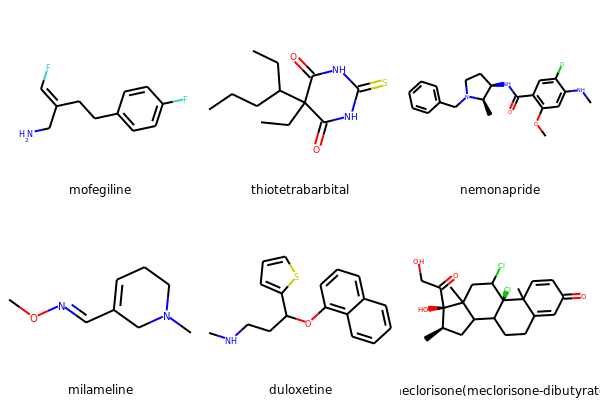
\includegraphics[width=0.75\textwidth,height=0.35\textheight]{images/random_molecules.png}
						\caption{Molecular Diagram of Random molecules from the Dataset}
						\label{fig:random_molecules}
					\end{figure}
				Using the RDKit Software library, we can extract the relevant ~chemical descriptors. For our dataset, 206 Chemical descriptors were extracted, shown below in table \ref{table:random_chem_descriptors}, are the same random molecules but with the first 5 descriptors displayed.
					\begin{table}[ht!]
						\caption{Chemical Descriptors of 6 Random molecules from the dataset}
						\centering
						\begin{tabular}{ | c | c | c | c |   }
							\hline
							Molecule Name & MinEStateIndex & ExactMolWt & NumValenceElectrons \\
							\hline
							Mofegiline & -0.2557111626 & 197.101605856 & 76 \\
							\hline
							Thiotetrabarbital & -0.9513194444 & 256.12454888 & 96 \\
							\hline
							Nemonapride & -0.1575794701 & 387.171354752 & 144 \\
							\hline
							Milameline & 0.9790277778 & 154.110613068 & 62 \\
							\hline
							Duloxetine & 0.1002371504 & 297.118735228 & 108 \\
							\hline
							Meclorisone(meclorisone-dibutyrate) & -1.6040011915 & 426.136464736 & 154 \\
							\hline
						\end{tabular}
						\label{table:random_chem_descriptors}
					\end{table}
				The beauty of the approach to the BBB problem is that from a statistical stand-point, we do not need a deep knowledge of Chemistry, we can simply make an educated neglect of the molecular names and the headers of the table \ref{table:random_chem_descriptors} and generate the matrix (rounded up to 3 decimal places ) shown as the feature vector \label{matrix:samp_feat_vec}
				\[ \left[ \begin{array}{c c c c}
					-0.256 & 197.102 & 76 & ... \\
					-0.951 & 256.125 & 96 & ... \\
					-0.158 & 387.171 & 144 & ... \\
					... & ... & ... & ...
				\end{array}
				\right]\]
				of size $2040 \times 206$, where 2040 is the number of molecules processed and 206 is the total number of chemical descriptors generated. This feature vector would then be utilised by the statistical processing techniques that would be described in the upcoming sections.
				\paragraph{Molecular Fingerprints as a Binary-Valued Feature Vector:}
				Another method of representing molecules is as a form of molecular fingerprint. Molecular Fingerprints are an abstract representation of molecular structure and properties of a given molecule in the form of a boolean array \cite{Jurgen2004}.
				The fingerprint representation is the result of applying a given kernel function to a molecule to generate an n-component bit vector. There are numerous types of formats for a molecular fingerprint; with the Morgan fingerprint (default fingerprint format for our prediction task) having a 2048 bit representation but the sizes of the vectors can vary depending on the kernel function used. \\
				The vector representation of a fingerprint is given by the general format
					\begin{equation}
						\vec{V_A} = (v_A(x_1), v_A(x_2),...,v_A(x_k),...,v_A(x_n))
					\end{equation}
				where $x_k$ indicates the absence or presence of a given feature \cite{Jurgen2004}. i.e
					\begin{equation}
						v_A(x_k) = 
						\begin{cases}
							1 & \text{Feature present} \\
							0 & \text{Feature absent}
						\end{cases}
					\end{equation}
				The table \ref{table:random_morgan_fingerprint} shows the transformation of a given molecule from our dataset into its SMILE format and then its fingerprint representation using the RDKit software library.
					%\begin{sidewaystable}
					\begin{table}[ht!]
						\centering
						\caption{Morgan Fingerprint representation of 2 Random molecules from the dataset}
						\begin{tabular}{ | c | c | c | c |   }
							\hline
							Molecule Name & SMILE & Molecular Representation & Morgan Fingerprint \\
							\hline
							111-trifluoro-2-chloroethane & C(CCl)(F)(F)F & 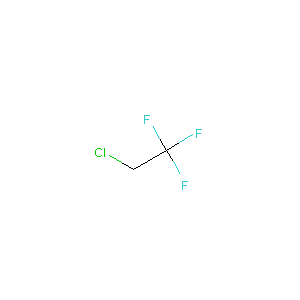
\includegraphics[width=2cm,height=2cm]{images/111-trifluoro-2-chloroethane.png} & [0.0, 0.0, 0.0, \ldots, 1.0, 0.0, 0.0, \ldots ,0.0, 0.0, 0.0] \\
							\hline
							Butanone & CCC(C)=O & 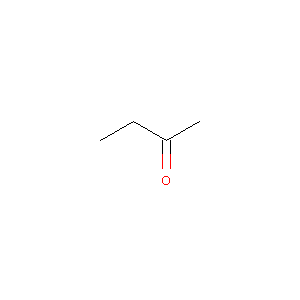
\includegraphics[width=2cm,height=2cm]{images/Butanone.png} & [\ldots, 1.0, 0.0, 0.0, 0.0, \ldots, 0.0, 0.0 ] \\
							\hline
						\end{tabular}
						\label{table:random_morgan_fingerprint}
					\end{table} 
					%\end{sidewaystable}
			\subsubsection{Similarity Measures} 
			\label{subsubsection_similarity_measures}
			The simplest way to cluster molecules together in a chemical database when performing virtual screening is through the concept of \textit{molecular similarity}. It is the core of Molecular Similarity Analysis (MSA) where the similarity measure, that characterizes the degree of proximity between pairs of molecules are manifested by their "molecular patterns", which are compromised of sets of features (chemical descriptors) \cite{Jurgen2004}. \\
			Many different molecular similarity measures exists and some are more suitable to certain virtual screening tasks than another, which is what prompts the discussion of molecular similarity measures in section \ref{subsubsection_similarity_measures}. 
			To determine the similarity between molecules, some form of similarity measure has to exist to compare molecules in the same representation. The similarity measures (similarity coefficient) are functions that maps pairs of compatible molecular representation into a real number. 
			
			For our prediction task, the main use of molecular similarity measures is in similarity searching when performing the nearest neighbour search. Here the molecules are ordered by their chosen chemical descriptors when we apply our similarity measure to calculate some form of structural relatedness between a target molecule and every other molecule in the dataset. The result is then a sorted list of molecules where the most similar molecules to our target molecule are located at the top of the list and in order of decreasing similarity.\\
			According to Jurgen \cite{Jurgen2004}, the most important components of similarity measures are
				\begin{itemize}
					\item \underline{The Representation}: Which is used to characterize the molecules that are being compared. An example would be molecular fingerprint representation of a molecule.
					\item \underline{The Weighing Scheme}: Used to assign differing degrees of importance to the various components of the molecular representation. An extra measure of accuracy in the weighing schemes would be the use of a chemical ontology database (e.g CheBL) when determining the importance of each component \cite{AnaPhd2014}.
					\item \underline{Similarity Coefficient}: A quantitative measure of the degree of structural relatedness between two molecules.
				\end{itemize}
			The main application of any similarity measure is to the fact that \textbf{structurally similar molecules exhibit similar properties} as stated by Johnson and Maggiora (1990) \cite{JohnMaggiora1990}. However, they also noted that an exception to the rule is that sometimes a small change in the structure of the molecule can result in a radical change in the properties that it exhibits. Which is why Ana Teixeira (2014) \cite{AnaPhd2014} notes that the use of a chemical ontology database would be a plausible method to combat this exception. For our prediction task, the exception to this rule is ignored for practical purposes as majority of molecules exhibit similar properties to one another.\\
			In similarity measure calculations, the most common measure for calculating fingerprint similarity is the Tanimoto coefficient, given by 
				\begin{equation}
				Tanimoto(\vec{v_i}, \vec{v_j}) = 
				\frac{\vec{v_i}\bullet\vec{v_j}}
				{\sum_{k}v_{ik} + \sum_{k}v_{jk} - \vec{v_i}\bullet\vec{v_j}  } 
				\end{equation}
			where $\vec{v_i}$ and $\vec{v_j}$ are the bit vectors for molecule $i$ and $j$. There are other similarity coefficients such as the Tversky and Dice but the Dice similarity measure was chosen for the k-nearest neighbour calculation of dataset.
	
	\section{Drug Design and Discovery}
	According to Dr A.N Boa \cite{hull2016}, the different stages of drug discovery are
		\begin{itemize}
			\item Programme Target Selection (Choosing the disease to work on)
			\item Identification and Validation of the drug target
			\item Assay Development
			\item Identification of a Lead Compound
			\item Lead Optimisation
			\item Identification of a drug candidate 
			\item Clinical Trials 
			\item Release of the drug 
			\item Follow-up Monitoring
		\end{itemize}
	Majority of the targets for the drugs we consume are usually proteins e.g enzymes, receptors and nucleic acids and the structure of the target is confirmed through a virtual screening method known as \textit{molecular docking}; it can be used to predict how the drug will bind to its target protein though various search/optimisation algorithms \cite{Jurgen2004}.
	Another Virtual Screening technique usually used is \textit{Quantitative Structure-Activity Relationships} (QSAR), here the underlying idea is that molecules with similar structures behave in the same way, as a result, the activity of a protein against a certain group of compounds is recorded and a QSAR model is the constructed from there and used to determine whether a given compound will bind to the target, thus screening the virtual compound library for drugs of interest.
	
	\section[CNS Drug Design and the Blood Brain Barrier]{Central Nervous System Drug Design and the Blood Brain Barrier}
	CNS Drugs aiming to pass through the Blood Brain Barrier often need to possess certain physical-chemical properties; some of which are Hydrogen bonding, ionization properties, molecular flexibility etc. \cite{Hassanetal2005}. The epithelial cells form an interface between the blood and the brain and these are commonly referred to as the Blood Brain Barrier. This interface occurs in other places within the body but what makes the BBB epithelial cells different are the tight junctions they form which makes it harder for drugs to pass through. Hassan and George (2005) further claim in their article that the majority of BBB penetration is through passive diffusion through the cellular membrane.
		\subsubsection{ADME Properties of CNS Drugs}
		For a CNS drug to be therapeutically effective, it must be easily disposed asides from having a high degree of potency. The ADME properties of a drug refers to its ability to be easily absorbed, distributed, metabolised and excreted. Some properties of CNS drugs affect their ADME properties, some of which are \cite{Hassanetal2005}:
			\begin{itemize}
				\item \underline{Solubility}: A drug must be very soluble in the blood and still be in high enough concentration at its target, in this case, the Blood Brain Barrier, so that it can easily be absorbed.
				\item \underline{Amount of Protein Binding}: Majority of CNS drugs tend to have high binding property towards proteins - this results in the drug being metabolised easily.
				\item \underline{Partition Coefficient (LogP)}: This is sometimes referred to as the \textit{lipophilicity} of the compound and has served as one of the most important factors in drug design. Higher lipophilicity results in drugs with higher metabolic turnover but lower solubility and absorption \cite{Hassanetal2005}. 
			\end{itemize}

	
	
\chapter{Machine Learning Classifiers}
	\textbf{Machine Learning} is a sub-field of Artificial Intelligence that involves the design of algorithms that can learn, make predictions and improve based on data without being explicitly programmed. There are 4 types of machine learning namely \cite{StephenM2014}
		\begin{itemize}
			\item \underline{Supervised Learning}: Here the machine learning algorithms are provided with training data where the correct outputs to the inputs are labelled and the algorithm learns to generalise from the training data.
			\item \underline{Unsupervised Learning}: This is the opposite of supervised learning, the training data contains only the inputs with no outputs; the algorithm then learns to generalise and cluster similar inputs together.
			\item \underline{Reinforcement Learning}: This lies in between supervised and unsupervised learning as no correct labels are provided to the training data, however, the algorithm is corrected when it makes a wrong prediction and it is required to iterate over numerous possibilities till it makes the correct prediction
			\item \underline{Evolutionary Learning}: This is a bio-inspired model where the concept of evolution is applied, numerous solutions are developed and are evaluated based on a fitness score. Models with higher fitness scores progress to the next training iteration whilst the lesser models are dropped till an optimal solution is found.
		\end{itemize}
	For the blood brain barrier (BBB) task, supervised learning techniques would be utilised for prediction purposes whilst the unsupervised learning techniques would be used for data exploratory purposes and to further understand and highlight patterns in the BBB dataset. The \href{http://scikit-learn.org/stable/}{Scikit-Learn} software library would be used extensively for the implementation of the supervised and unsupervised learning models.
	
	\section{Data Representation and Preprocessing}
	The \href{http://pandas.pydata.org/}{Pandas} and \href{http://www.numpy.org/}{Numpy} libraries are used throughout the project and they are also the underlying library used by Scikit-Learn. 
		\begin{listing}[!htbp]
			\inputminted[breaklines=true,breakautoindent=true,linenos=true]{python}{source_code/dataset.py}
			\caption{Functions to load, preprocess and transform the dataset}
			\label{code:dataset_preprocess}
		\end{listing}
	In code listings \ref{code:dataset_preprocess}, the training data is loaded in using Numpy and then converted into the RDKit molecular format; the failed indices are recorded and deleted from the Numpy array and the resulting data is then transformed based on their chemical descriptors and stored in a Numpy array for use by the supervised and unsupervised models.
	
	It is worth noting the dataset used is a highly biased one; After preprocessing and cleaning, there are a total of 1563 molecules that pass through the blood brain barrier and a total of 477 molecules that do not pass through the barrier. This bias would be accounted for during the training phase as the machine learning classifiers would be cross validated as explained in the model evaluation section.
	
	
	
	
	
	\section{Unsupervised Learning}
	Before training the classifiers with the preprocessed data; it is usually best to carry out some form of exploration into the dataset to enable educated guesses about the best machine learning models to utilise for the prediction task. In this section, unsupervised learning techniques would be used to gain insights into the bbb dataset with the aim being to determine if it is possible to linearly fit a classifier symbolically to divide between the molecules that pass through the barrier and the ones that do not. The main areas focused on would be the transformation of the dataset using the Manifold learning algorithms and the clustering of the data points.
	
		\subsection{Principal Component Analysis (PCA)}
		\textbf{Principal Component Analysis (PCA)} is a form of dimensionality reduction technique that aims to reduce the number of dimensions of the data mainly for visualisation purposes whilst still preserving the statistical meaning of the data and reducing the number of important (principal) components; Here only a small subset of the features of the data are selected according to how important they are; 
		
		To illustrate further using the feature vector shown in \ref{matrix:samp_feat_vec}, the vector has a dimensional size of 206 features, as all the 2040 molecules have a chemical descriptor size of 206. Plotting a single molecule on a graph with 206 dimensions would be nearly impossible as 2D and 3D data are the best ways to illustrate statistical data for humans. By applying the Principal Component algorithm to the feature vector, it proceeds to find the direction of maximum variance for each molecule that is, it returns a new vector that contains the most information. The directions of maximum variance returned are referred to as the \textit{principal components}.
		
		In order to gain a deeper understanding of our data, the PCA algorithm is applied with the number of principal components set to 2 i.e (n\_components = 2). In the 2D representation shown below in figure \ref{fig:scatter_pca_2D}, the data points are tightly clustered in the middle, and whilst this looks like it is linearly inseparable, with some clustering techniques that would be shown later, a better representation where it is more distinguishible between the data points would be shown.
		\begin{figure}[H]
			\centering
			\includegraphics[width=\textwidth,scale=1,totalheight=0.5\textheight]{images/scatter_pca}
			\caption{2D Scatter Plot after applying the PCA Algorithm}
			\label{fig:scatter_pca_2D}
		\end{figure}
	
		To further examine the data, the next 3 principal components are selected to create a 3D plot. The 3D plot as shown in figures \ref{fig:scatter_pca_3D} and \ref{fig:scatter_pca_3D_2} also has the same clustering of a significant proportion of the blue molecules in the same space as the red molecules but looks more linearly separable than the 2D plot. This highlights that would a little bit of feature engineering, it would be possible to seperate the data points into 2 clusters of red and blue i.e molecules that pass through the barrier and the ones that do not. 
		\begin{figure}[H]
			\centering
			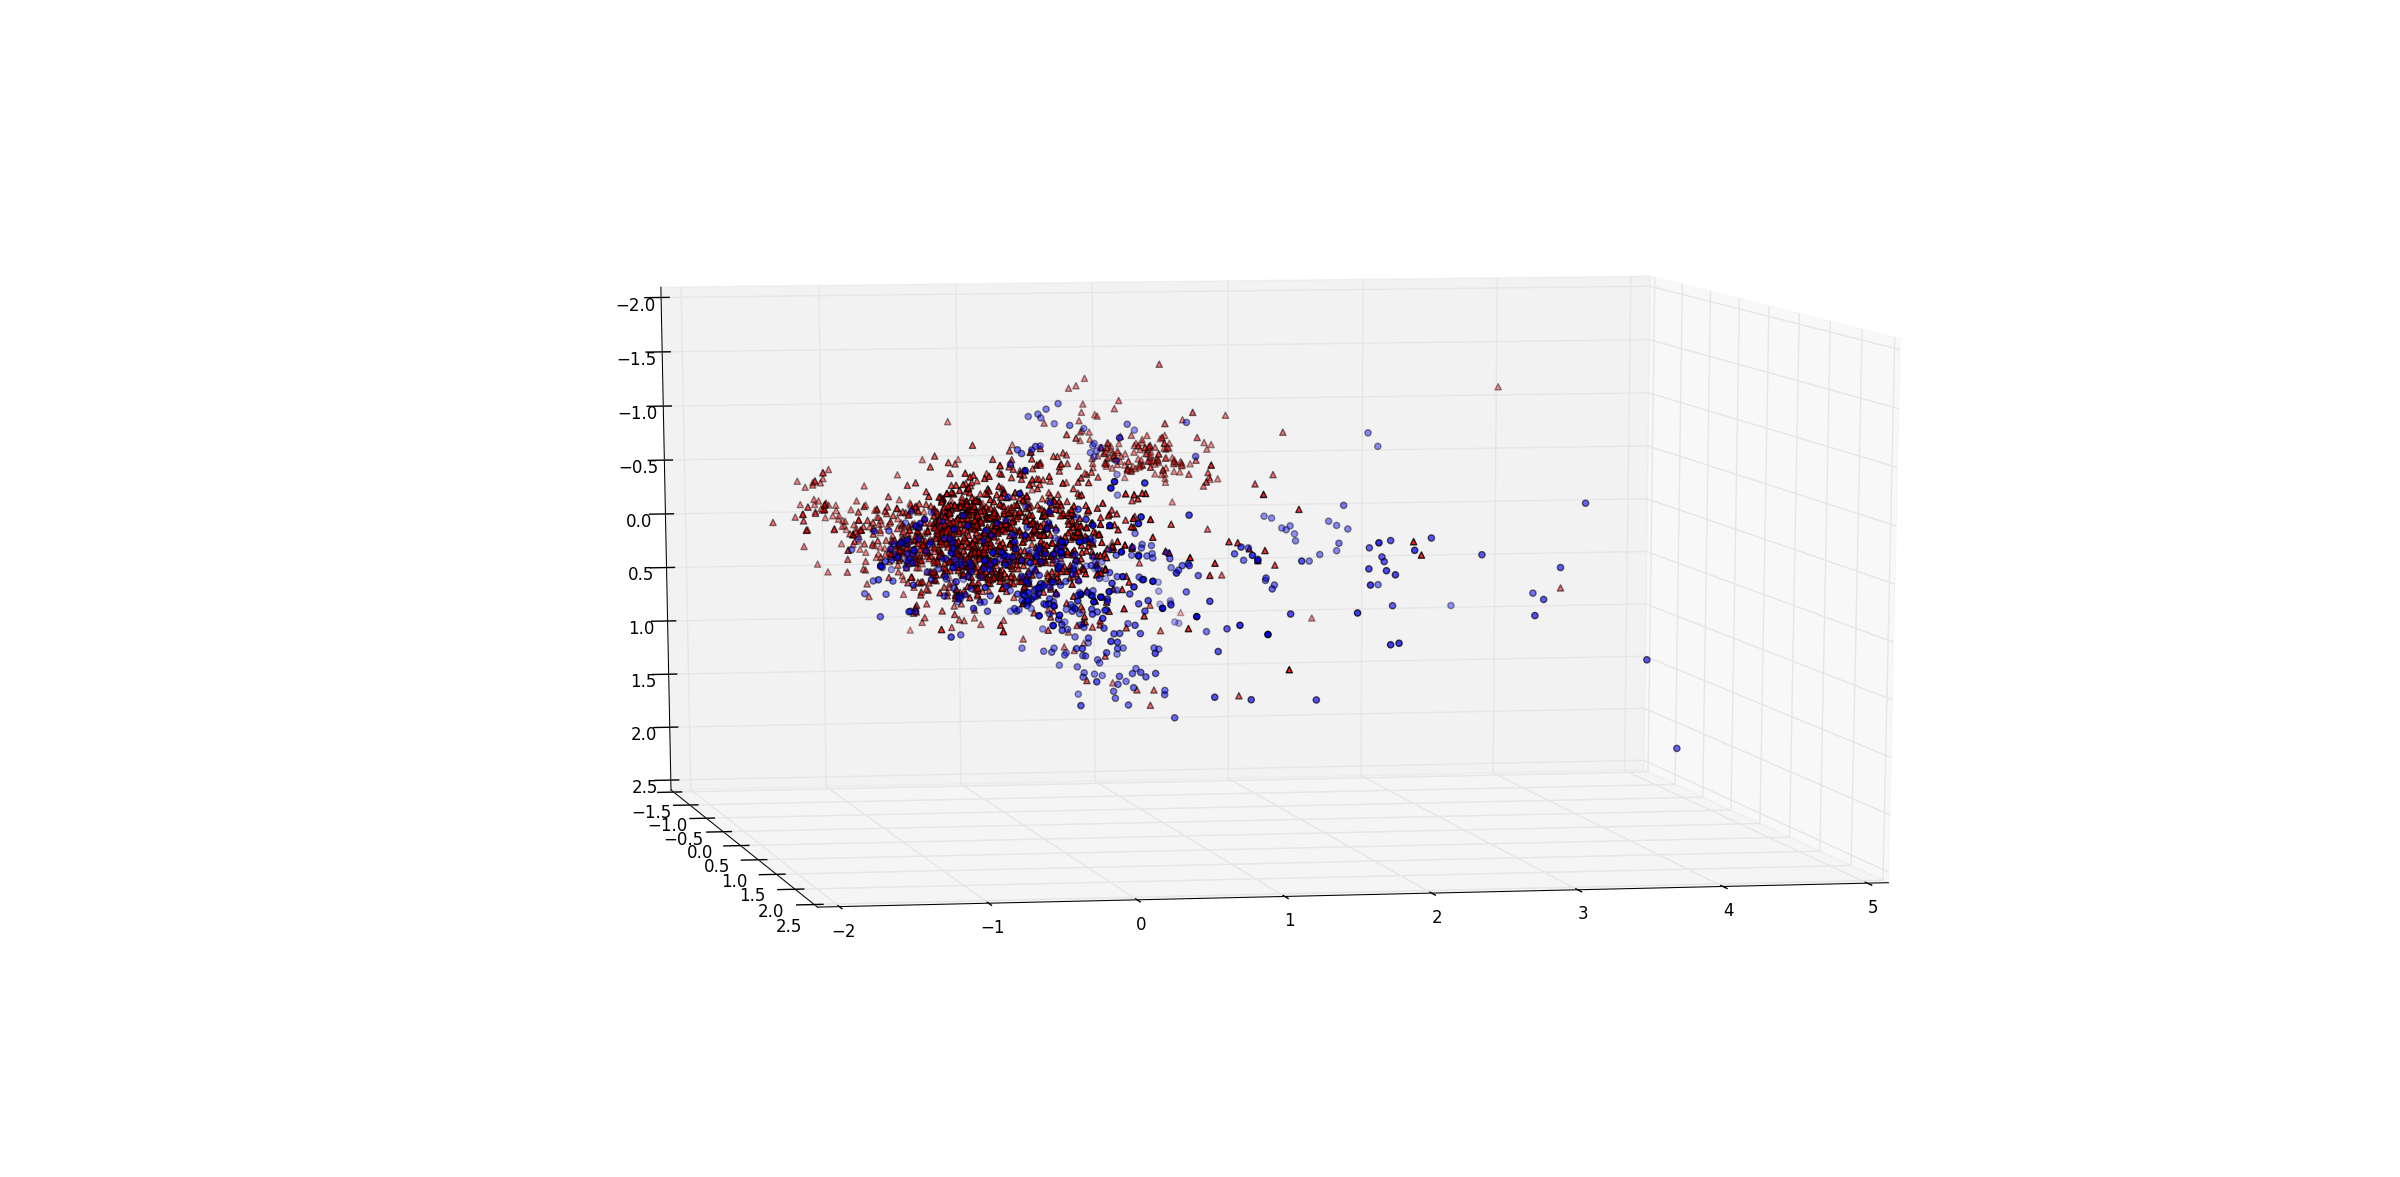
\includegraphics[width=\textwidth,scale=1,totalheight=0.4\textheight]{images/scatter_pca_3D}
			\caption{3D Scatter Plot after applying the PCA Algorithm (I)}
			\label{fig:scatter_pca_3D}
		\end{figure}
		\begin{figure}[H]
			\centering
			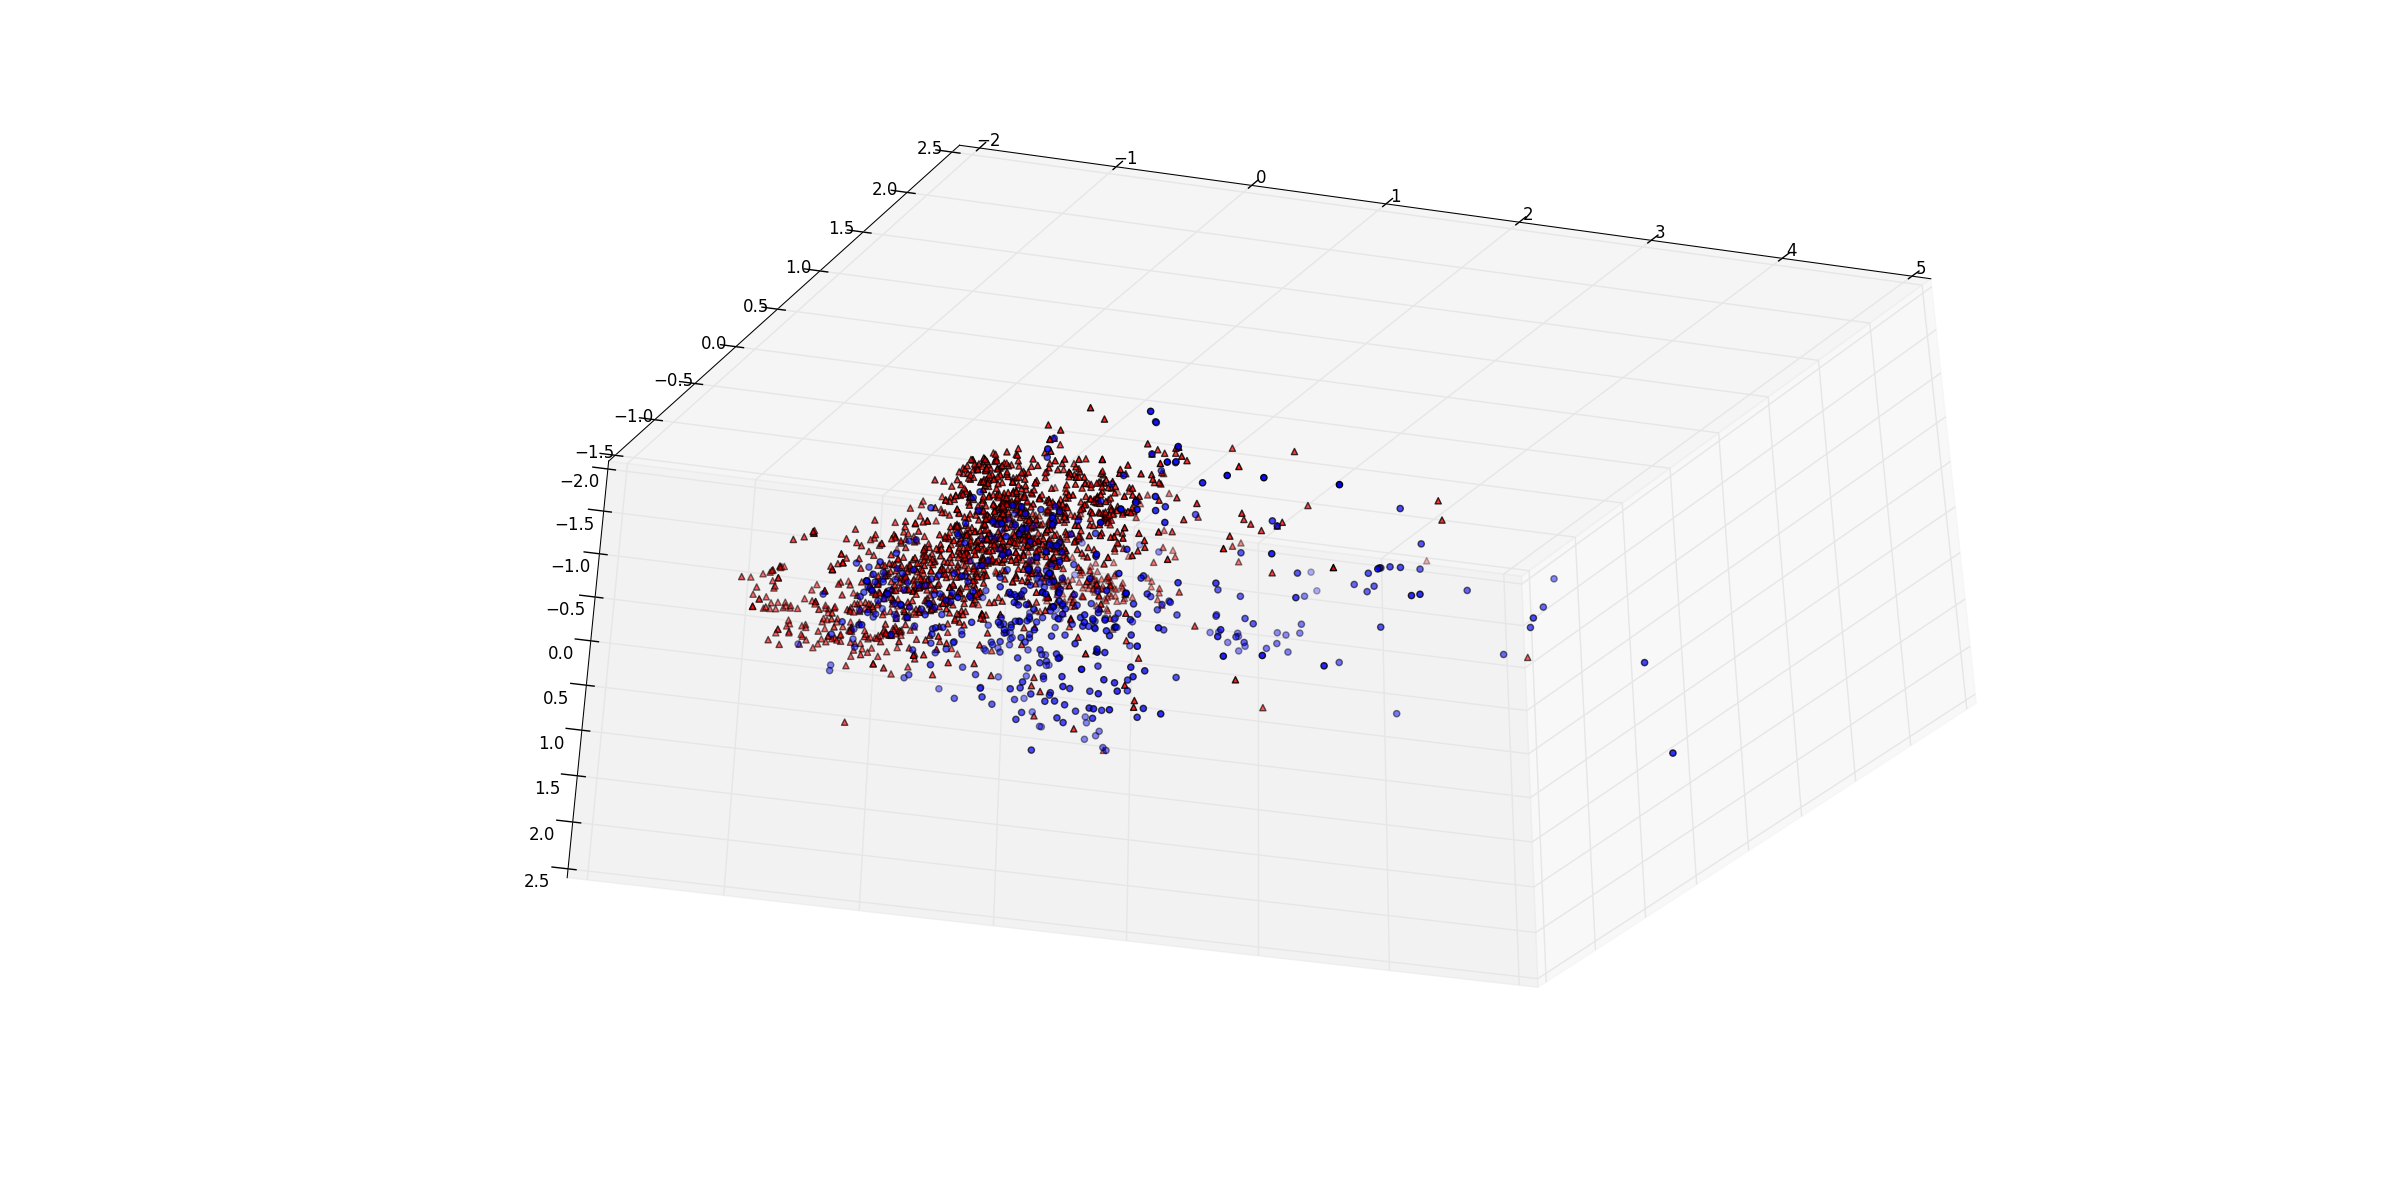
\includegraphics[width=\textwidth,scale=1,totalheight=0.4\textheight]{images/scatter_pca_3D_2}
			\caption{3D Scatter Plot after applying the PCA Algorithm (II)}
			\label{fig:scatter_pca_3D_2}
		\end{figure}
		
		A major benefit of exploratory data anlysis as we have seen here is that it is worth gaining insights into the dataset to determine the kind of feature engineering required to achieve high performing machine learning models.
	
	
	
		\subsection{Manifold Learning with t-SNE}
		\paragraph{Manifold Learning algorithms} are also another form of dimensionalty reduction techniques similar to the Principal Component Analysis algorithm. The t-SNE algorithm, a manifold learning technique, would also be used to further visualise the data in another attempt to further see if it is visually possible to separate between the molecules that do and do not pass through (the red and blue dots). 
		
		Manifold Learning Algorithms excel at data visualisation tasks, they provide more complex mappings and often better data representations but perform poorly for data classification tasks. They perform poorly because they do not allow transformations of new data once they have been fitted \cite{Yairetal2008}.\\
		
		The t-SNE algorithm is used because it tries as much as possible to maintain the distance between the data points in the original feature vector space during transformation; This way the feature vector can be transformed and reduced to better suit our data exploratory purposes whilst still preserving the integrity of the data. It puts more emphasis on points that are close by rather than preserving points that are far apart \cite{Mueller2016}.
		\begin{figure}[H]
			\centering
			\includegraphics[width=\textwidth,scale=1,totalheight=0.4\textheight]{images/scatter_tsne}
			\caption{2D Scatter Plot after applying the t-SNE Algorithm (Molecular Descriptor dataset)}
			\label{fig:scatter_tsne_2D}
		\end{figure}
		Looking at the t-SNE scatter plot, there is a small cluster of the molecules that do not pass through (B) at the top and some randomly distributed throughout the plot, whilst the ones that pass through the BBB barrier (A) maintain an even distribution around the feature space. This result is to be expected as the data is biased towards molecules that cross the barrier and it also hints at the fact that the molecules that do not cross the barrier might share a lot in common with molecules that cross the barrier.
		\begin{figure}[H]
			\centering
			\includegraphics[width=\textwidth,scale=1,totalheight=0.5\textheight]{images/scatter_tsne_mfps}
			\caption{2D Scatter Plot after applying the t-SNE Algorithm (Morgan Fingerprint dataset)}
			\label{fig:scatter_tsne_mfps_2D}
		\end{figure}
		The scatter plot has no significant difference with the Morgan Fingerprint dataset, it highlights the clusters of the B molecules more visibly. Further analysis would need to be carried to create a more linear separable representation.
		\begin{figure}[H]
			\centering
			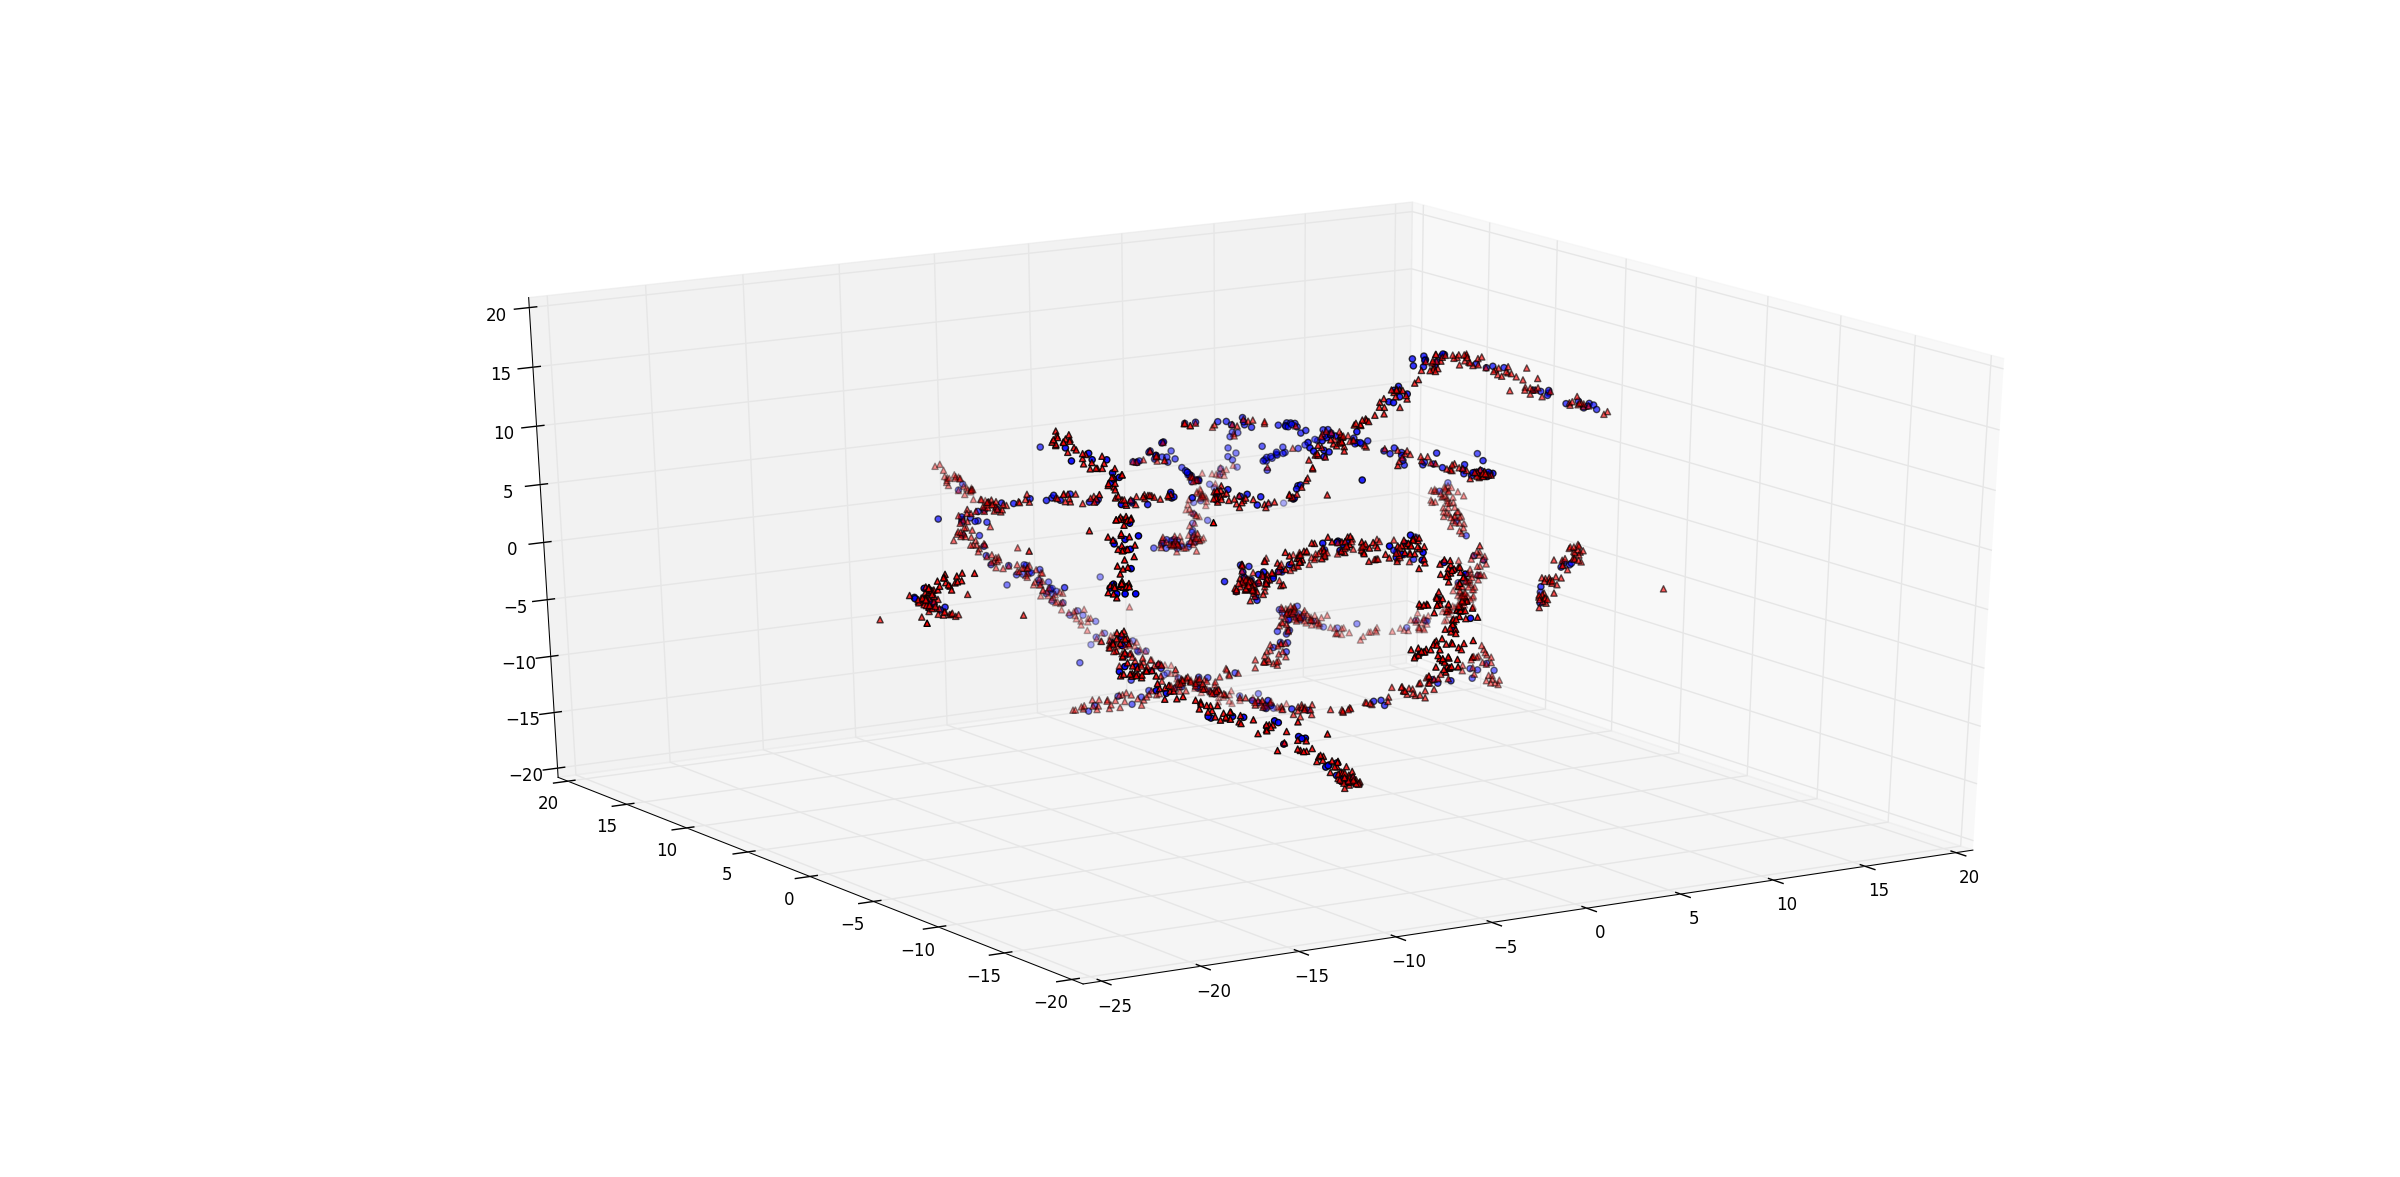
\includegraphics[width=\textwidth,scale=1,totalheight=0.5\textheight]{images/scatter_tsne_3D}
			\caption{3D Scatter Plot after applying the t-SNE Algorithm (Molecular Descriptor dataset)}
			\label{fig:scatter_tsne_3D}
		\end{figure}
		The 3D scatter plot of the simple molecular descriptor data looks slightly more separable than its 2D counterpart.
		
		
		
		
		
		
		
		\subsection{Clustering}
			\subsubsection{K-Means Clustering}
			In our further attempts to have some form of linearly separable data, we further explore clustering techniques. Here, the 2 principal components of our feature vector are selected and applied to the k-means clustering algorithm.
			
			The K-means algorithm, also known as \textit{Lloyd's algorithm}, aims to find cluster centroids that are representative of regions within the dataset or feature vector. The algorithm selects the approximate center of the clusters and iteratively assigns each data point to this center, and then sets the cluster center again as the average of the data points in the cluster using the equation \ref{equa:kmeans}.
				\begin{equation}
					\label{equa:kmeans}
					\sum_{i=0}^{n}min_{\mu_{j} \in C}(||x_{j} - \mu_{i}||^{2})
				\end{equation}
			where $\mu_{j}$ is the mean of the cluster, $C$ is the cluster, $x_{j}$ is the current data point and $\mu_{i}$ is the current mean of the calculation \cite{Sculley2010}.
			It repeats this process until the cluster centroids do not change significantly.
			%\begin{figure}[H]
				%\centering
				%\includegraphics[width=\textwidth,scale=1,totalheight=0.4\textheight]{images/kmeans_smd_scatter}
				%\caption{2D Scatter Plot found by k-means on Simple Molecular Descriptors. \textit{Original data points on the right and clusters found on the left}}
				%\label{fig:kmeans_smd_scatter}
			%\end{figure}

			Applying the algorithm to a feature vector derived from the Morgan fingerprint dataset. We now have a visualisation showing two clusters with their centroids in yellow, shown in figure \ref{fig:kmeans_morgan_scatter}. This is a more linearly separable diagram as the molecules that pass through the barrier shown in red are clustered around their centroid and also the molecules that do not pass through.
			\begin{figure}[H]
				\centering
				\includegraphics[width=\textwidth,scale=1,totalheight=0.4\textheight]{images/kmeans_morgan_scatter}
				\caption{2D Scatter Plot found by k-means on fingerprint dataset. \textit{Original data points on the right and clusters found on the left}}
				\label{fig:kmeans_morgan_scatter}
			\end{figure}
			
			
			\subsubsection{Agglomerative Clustering}
			These are a form of hierarchial clustering techniques with major applications in natural language processing. Hierarchial techniques form clusters by continuously merging or splitting data points till it meets the required number of clusters. Agglomerative clustering works in a similar manner where each data point is a cluster of its own and iteratively the algorithm merges the clusters togethers using a \textit{merging strategy}. 
			
			The merging strategy used for our dataset was the \textbf{Ward Strategy}, where the algorithm minimises the sum of squared differences within all the clusters, which is similar in a way to the K-Means algorithm.
			
			Figures \ref{fig:agg_smd_scatter} and \ref{fig:agg_morgan_scatter} show the result of applying the algorithm to a feature vector derived from the two principal components of the simple molecular descriptors and the morgan fingerprint descriptors. 
			%For the Simple Molecular dataset, the entire dataset was scaled to have a minimum of -1 and a maximum of 1. Then the 2 principal components were selected, a ward agglomerative cluster algorithm was applied and it created 2 clusters with cluster 1 having 1442 samples and cluster 2 having 598 samples. The original dataset had 1563 molecules passing through the barrier and 477 molecules not passing through, most likely cluster 1 represents the molecules that pass through
			\begin{figure}[H]
				\centering
				\includegraphics[width=\textwidth,scale=1,totalheight=0.4\textheight]{images/agg_smd_scatter}
				\caption{2D Scatter Plot of clusters found by the agglomerative ward algorithm on the simple molecular dataset}
				\label{fig:agg_smd_scatter}
			\end{figure}
			%Applying the same cluster to the Morgan fingerprint dataset, without preprocessing the data, it created 2 clusters; cluster 1 with 1894 samples and cluster 2 with 146 samples. The simple molecular descriptor dataset proves to be a better dataset for this clustering algorithm as it achieves a lower error rate
			With the blue circles being the molecules that pass through the barrier and the triangles being the molecules that do not pass through the barrier.
			\begin{figure}[H]
				\centering
				\includegraphics[width=\textwidth,scale=1,totalheight=0.4\textheight]{images/agg_morgan_scatter}
				\caption{2D Scatter Plot of clusters found by the agglomerative ward algorithm on the Morgan Fingerprint dataset}
				\label{fig:agg_morgan_scatter}
			\end{figure}
			



	\section{Machine Learning Models}
		\subsection{K-Nearest Neighbours}
		K-Nearest Neighbours (k-NN) is a form of instance based learning; Instanced-based learning techniques store the training example in memory and utilise them to make predictions. All data points (nearest neighbours) in the feature vector are defined in a form of euclidean space; where a prediction for an instance is made by finding its euclidean distance to its nearest $k$ neighbours. 
		
			\begin{mdframed}[]
				\paragraph{The k-NN training and classification Algorithm \cite{Mitchell1997}}
				\begin{itemize}
					\item \textbf{Training Algorithm}
					\\ For each training example $v$, add it to the list of \textit{training\_examples}
						\begin{itemize}
							\item Ensure the elements of the training sample are sorted using the distance function
								\begin{equation}
									d(x_i,x_j) \equiv \sqrt{\sum_{r=1}^{n}(a_r(x_i) - a_r(x_j))^2} 
								\end{equation}
							where $a_r(x)$ denotes the $r$th attribute of instance $x$ and $x_i,x_j$ are two arbitrary instances to be compared
						\end{itemize}
					
					\item \textbf{Classification Algorithm} 
					\\ Given a query instance $x_{q}$ to be classified
					\begin{itemize}
						\item[] Let $x_1,\dots,x_k$ represent $k$ instances from the \textit{training\_example} that are nearest to $x_q$.
						
						\item Return the class of $x_q$ denoted by $\hat{f}(x_q)$; given by
							\begin{equation}
								\hat{f}(x_q) \leftarrow argmax_{v \in V} \sum_{i=1}^{k} \partial (x_i)
							\end{equation}
						where $V$ is set of all possible classes an instance $x$ can belong to and $\partial(x_i)$ represents the class of the current instance $x_i$ from the $k$ instances.
					\end{itemize}
				\end{itemize}
			\end{mdframed} 
		
		Applying the k-NN algorithm to the simple molecular dataset yields the results shown in figure \ref{fig:knn_smd}. The reduction in training accuracy as the number of neighbours increases is a good indicator that the model is not overfitting; Overfitting occurs when the model memorises the training data instead of learning the statistical patterns within them.
		\begin{figure}[H]
			\centering
			\includegraphics[width=\textwidth,scale=1,totalheight=0.5\textheight]{images/knn_molecular_descriptors}
			\caption{k-NN classifier for 10 neighbours using the Simple Molecular Descriptors}
			\label{fig:knn_smd}
		\end{figure}
		The algorithm is also applied to the morgan fingerprint dataset, shown in figure \ref{fig:knn_mfps}. There is little or no improvement in accuracy between both datasets with the number of neighbours at 10
		\begin{figure}[H]
			\centering
			\includegraphics[width=\textwidth,scale=1,totalheight=0.5\textheight]{images/knn_morgan_dice_fingerprint}
			\caption{kNN classifier for 10 neighbours using the Morgan Fingerprint dataset}
			\label{fig:knn_mfps}
		\end{figure}
		
		
		
		\subsection{Support Vector Machines}
		Support Vector Machines (SVMs) are a set of supervised learning techniques that make predictions by learning the statistical hyper-plane (support vectors) that determines the categories of data in the input space. They are very effective in high dimensional situations as is the case with our dataset (2048 x 206) and also very memory efficient; as only a subset of the training points in the decision function i.e support vectors are stored in memory. 
		
		SVMs are computational intensive and as a result, they do not scale well with large datasets; The driving idea behind SVMs is to infer the hyper-plane that divides the data into categories. Applying this to our BBB dataset, the goal is to have the SVM learn the support vectors that classify a molecule as either positive (passes through the barrier) or negative. Figure \ref{fig:svm_mol} shows the result of applying the SVM classifier to the simple molecular dataset.
		%Scaling the data using a Standard Scaler and selecting the top 100 principal component, a mean accuracy of 84.9\% was achieved using both datasets
		\begin{figure}[H]
			\centering
			\includegraphics[width=\textwidth,scale=1,totalheight=0.4\textheight]{images/mol_decision_svm}
			\caption{Support Vector Machines with different kernel functions on Simple Molecular Dataset}
			\label{fig:svm_mol}
		\end{figure}
		
		The figures show the algorithm applied on our datasets using numerous kernel functions. Kernel functions are basically a form of similarity functions, they compute the distances between data points in the input space. To enable the SVM classifier make predictions for a new data point, its distance to the support vectors are calculated using any of the kernel functions (linear, polynomial, sigmoid or Radial Basis function (RBF)) \cite{StephenM2014}. Due to the highly mathematical nature of these kernel functions, their intricate details can be safely ignored and their classification results instead focused on for our BBB classification tasks. 
		
		\begin{figure}[H]
			\centering
			\includegraphics[width=\textwidth,scale=1,totalheight=0.4\textheight]{images/fps_decision_svm}
			\caption{Support Vector Machines with different kernel functions on Morgan Fingerprint Dataset}
			\label{fig:svm_fps}
		\end{figure}
		
		
		
		
		\subsection{Decision Trees}
			Decision trees are an example of non-parametric supervised learning algorithms; The aim of the algorithm is to have a model that can classify an input data (feature vector) based on simple rules the algorithm has inferred from the features of the dataset. Here observations learnt from the dataset are represented in branches (decision boundaries), which then lead to classifications of the input represented in the leaves. 
			
			To illustrate further, an example from the BBB classification is shown in figure \ref{fig:bbb_tree_smd_detailed}. The overview of the algorithm is that it learns the necessary if/else questions to classify an input.
				\begin{figure}[H]
					\centering
					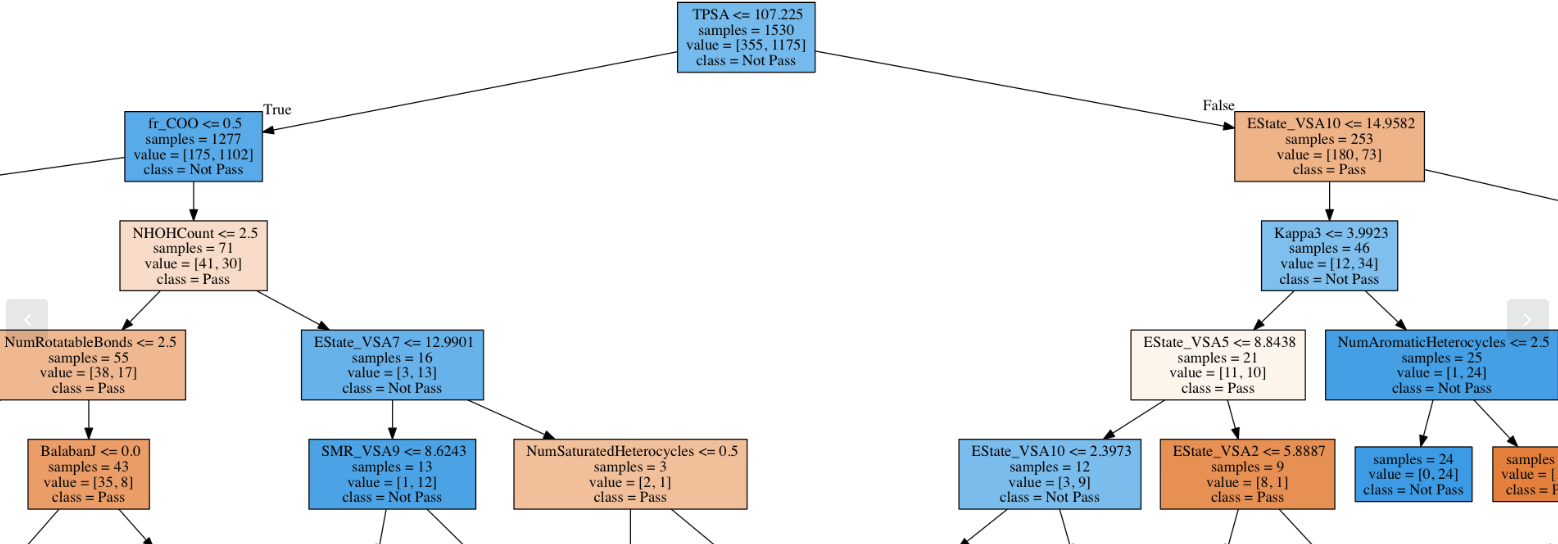
\includegraphics[width=\textwidth,scale=1,height=0.5\textheight]{images/bbb_tree_smd_larger}
					\caption{Decision Tree}
					\label{fig:bbb_tree_smd_detailed}
				\end{figure}
			Here in figure \ref{fig:bbb_tree_smd_detailed}, the algorithm performed a search over all the training data and picked \textit{TPSA} (total polar surface area) as the most informative variable in deciding whether a molecule passes through the barrier or not; Splitting the tree into 1277 molecules that do not pass and 253 molecules that pass. The algorithm then recursively searches each branch and further creates more branches till it reaches a node (leaf) that contains a single target value (target classification).
			
			Figure \ref{fig:bbb_tree_smd} shows the generated tree after applying the decision tree algorithm to our simple molecular dataset; With the algorithm achieving an accuracy of $\sim85\%$ on the simple molecular dataset.
				\begin{figure}[H]
					\centering
					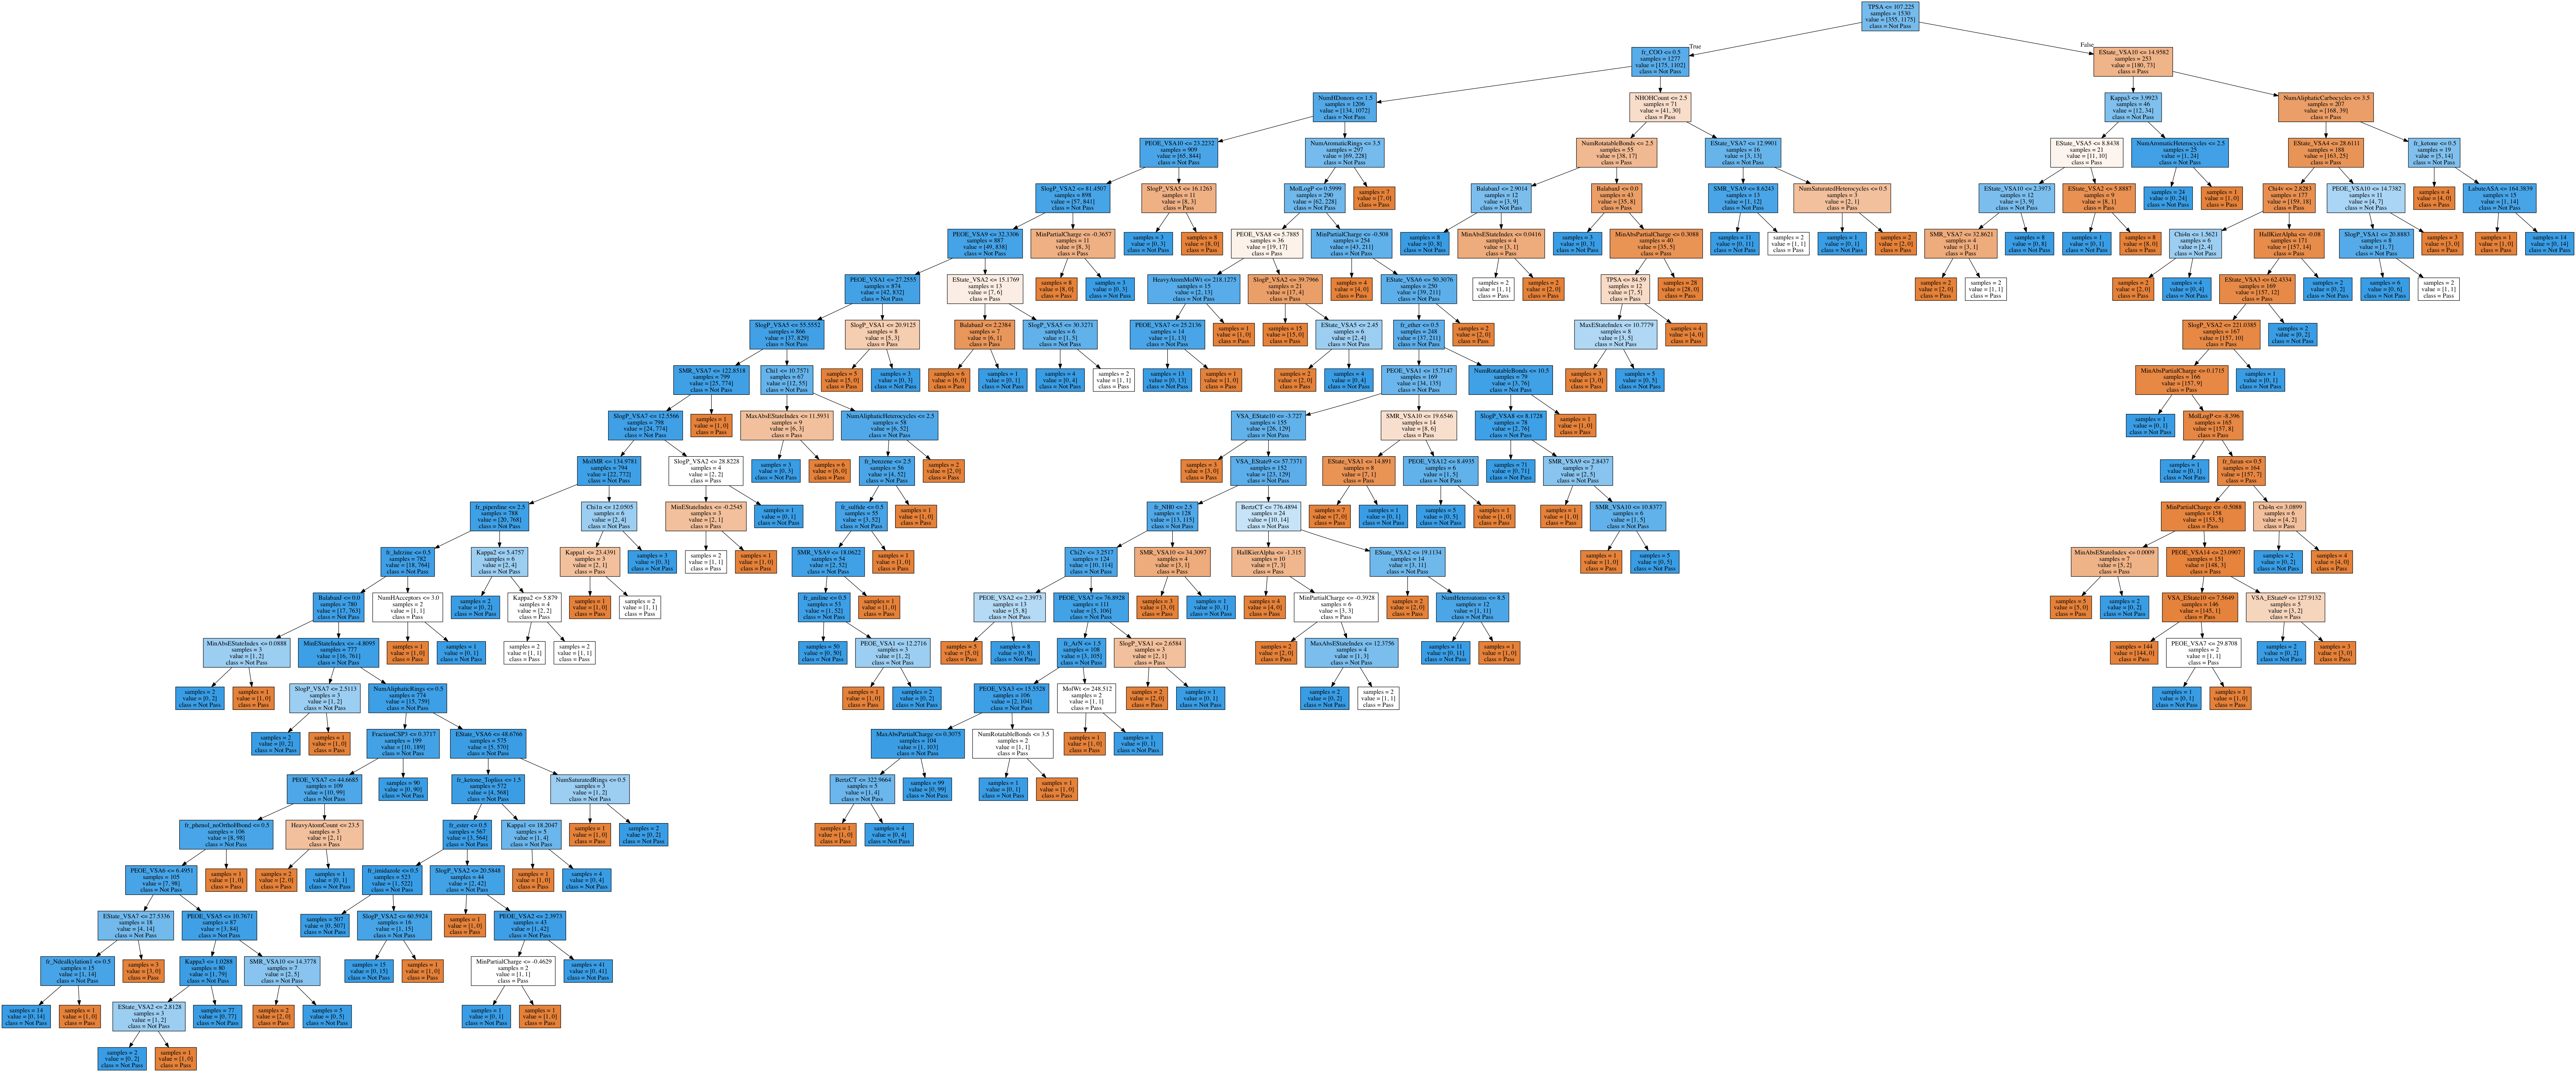
\includegraphics[width=\textwidth,scale=1,totalheight=0.4\textheight]{images/bbb_tree_smd}
					\caption{Decision Tree: Simple Molecular Descriptors}
					\label{fig:bbb_tree_smd}
				\end{figure}		
			
			\paragraph{Ensembles of Decision Trees}
			Ensembles in the context of machine learning refers to the combination of numerous machine learning models to create a more powerful model. This technique would be utilised in section \ref{subsection:ensemble}, where all the machine models that would be discussed will be combined to create an even more powerful and stable model.
			
			Decision trees tend to overfit and learn the rules only in the training data and perform poorly when presented with new data \cite{Mueller2016}. To overcome this problem, numerous decision trees would be combined to create an ensemble of decision trees: random forests, gradient boosted decision trees, extra trees and Adaboost decision trees.
			\subsubsection{Random Forests}
			Random forests are an ensemble of decision trees where each decision tree has been trained with a subsection of the dataset with the knowledge that the said tree would overfit on that part of the dataset. The overfitting of the random forest is reduced by averaging the result from all the individual trees to return a classification.
			
			An accuracy of $\sim87\%$ was achieved using the random forest classifier on the simple molecular descriptor dataset whilst an accuracy of $\sim89\%$ was achieved on the Morgan fingerprint dataset;With the number of trees in the random forest set to 20.
				
			\subsubsection{Extremely Randomized Trees}
			Extremely randomized trees also known as \textit{Extra Trees} are very similar to Random Forests. The difference between them is that at each step of the algorithm the entire dataset is used as opposed to partial datasets in random forests and the decision boundary is also chosen at random instead of the best one \cite{Pierre2006}.
			
			The extra trees algorithm performed slightly better than the random forests algorithm; On the simple molecular dataset, the extra trees score an accuracy of $\sim90\%$ and on the Morgan fingerprint dataset, the extra trees score an accuracy of $\sim89\%$, performing just slightly less than the random forest on the same dataset with the number of extra trees was set to 20.
			
			\subsubsection{Gradient Tree Boosting}
			Gradient boosted trees differ from random forests in the sense that in gradient tree boosting, very small trees called \textit{weak learners} are trained serially where the current tree learns from the mistakes of the previous tree. The weak learners usually have a shallow dept of 5 and can therefore make faster predictions. The learning rate is also another parameter of the gradient boosted trees that can be optimised; the learning rate is the degree to which the current tree learns from its predecessors \cite{Mueller2016} with a higher rate resulting in stronger corrections.
			
			Applying the gradient boosted trees algorithm to both derivations of our dataset with
			the number of estimators set to 150 and the learning rate to 0.45. An accuracy score of $\sim86\%$ was achieved on the simple molecular descriptors and $\sim82\%$ on the Morgan fingerprint dataset.
				
			%\subsubsection{AdaBoost Decision Trees}
			%Applying the AdaBoost algorithm to the decision trees, an accuracy of $\sim83\%$ was achieved on the simple molecular descriptor dataset, and an accuracy of $\sim81\%$ on the Morgan fingerprint dataset. Both rounds of classification with number of trees = 200. Strangely, the Adaboosted decision trees ought to provide better results than the random forest or extra trees classifiers. 
		
		
		\subsection{Neural Networks(Notes)}
				%The Human brain is a very fascinating and robust system, the basic processing unit of the brain is the nerve cell or neuron and there are around 100 billion neurons in the brain all connected together by synapses. These neurons are electrically excitable, they pass signals from one neuron to the next by electrical and chemical signals when the membrane potential reaches some threshold, which can be inhibited if the threshold is not exceeded. 
			A Neural Network is a computational model inspired by the human brain, it consists of a network of neurons connected together by axons. The inspiration behind the model is that if learning occurs in the brain and if we can represent this in a computational model then we can achieve some form of intelligence in our systems.
				%\paragraph{Hebbian Learning}
				%This is a learning concept of the brain based on the mechanism neural plasticity proposed by Donald Hebb. The rule formulated states that changes in the strength of synaptic connections are proportional to the correlation in the firing of the two connecting neurons, the strength of the connection is proportional to the frequency of excitement between them. However, the connection between two neurons that never fire will eventually be broken. \\
				%The idea of repetition enhances retention can also be applied here, where actions that are repeated continuously will create retention in the brain \cite{Cunninghametal1984}. An example is in the experiment carried out by Ivan Pavlov, where his dogs were conditioned to associate the ringing of a bell to the presence of food. As a result, the neurons responsible for salivating over food and for hearing the bell would have a very strong connection to the extent that merely hearing the bell was sufficient to cause the salivating neurons to fire. 
			\subsubsection{Multi Layer Perceptron}
			The Perceptron can also be referred to a collection of neurons along with a vector of inputs and a vector of weights to fasten the inputs to the neuron. This neuron in this network consists of its inputs, weights, threshold and activation function. Each neuron,receives an input along with the strength of the input i.e weight, which it multiplies together and if the value is greater than the threshold, the neuron fires. \\
			For our dataset the input $X = [x_1,x_2,x_3,...,x_n]$ to a Perceptron could be either a simple molecular feature vector value e.g the number of hydrogen atoms in the molecule or vectors of 1s and 0s if we're using the Morgan fingerprint dataset to train the network. Each neuron is also given a vector of small random positive and negative values as its weights. The neuron calculates its activation value as 
				\begin{equation}
				h = \sum_{i=1}^{m}w_ix_i
				\end{equation}
			This activation value is then passed on to the activation function $f(h)$ which fires if the activation value is greater than the threshold. A threshold value of 0 was used irrespective of the training dataset. The output value of the function is given by
				\begin{equation}
					output = f(h) = 
					\begin{cases}
					1 & \text{if h} \textgreater \theta \\
					0 & \text{if h} \le \theta
					\end{cases}
				\end{equation}
			\paragraph{Multi Layer Perceptron}
			The Input layer to the neuron is the same as the length of the feature vector plus one (the fixed bias input) as shown in figure \ref{fig:mlp}. For the simple molecular feature dataset, the number of inputs $n$ to the network is 206, as that is the number of simple chemical descriptors that were calculated. For the Morgan Fingerprint dataset, $n = 2048$ where $n$ represents the length of the bit vector. 
			
			The bias input is used as a control value to adjust the value that the neuron fires at. An example is when the feature vector to a neuron is all zeros and the neuron should fire. By our activation function, the neuron wouldn't fire because its activation value does not exceed the threshold. By adding a fixed value (bias) of $\pm1$ to the feature vector, we can then adjust the weight to make the neuron fire or not.
				\begin{figure}[H]
					\centering
					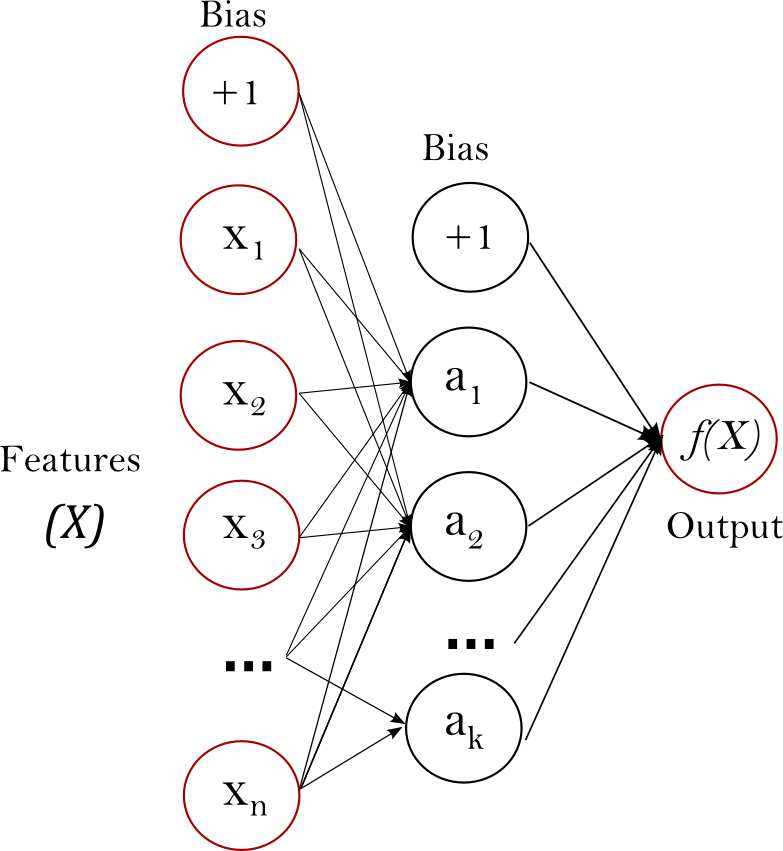
\includegraphics[width=0.9\textwidth,scale=1,totalheight=0.5\textheight]{images/multilayerperceptronnetwork}
					\caption{Multi Layer Perceptron \cite{ScikitLearn2016}}
					\label{fig:mlp}
				\end{figure}
			\subsubsection{Application to the Blood Brain Barrier prediction}
			%We are undertaking a form of supervised learning in the BBB prediction. The dataset we have compiled is labelled with the correct class and this data is fed to the neural network in order for the it to generalise what it has learned about our data. The network will then find patterns in the molecules that cross the blood-brain barrier and predict if an unknown molecule will cross it or not. \\
			Let $X = [x_1,x_2,x_3,...,x_n]$ be the input vector to our network for $n$ features and $W=[w_1,w_2,w_3,...,w_n]$ the weights. Each neuron calculates whether it should fire or not based on its activation vector. We then examine the wrong neurons i.e the neurons that fired when they should have not. Figure \ref{fig:neural_net_activation} shows the activations of the neurons in the first layer of the neural network during the training phase with the darkest color representing no activation.
			
			For each wrong neuron $i$, we calculate the difference in weights for it $\Delta w_i = -(y_i - t_i) * x_i$ where $y_i$ is the output and $t_i$ is the target output, the weight for neuron $i$ is then updated as $w_i = w_i + \Delta w_i\eta$, where $\eta$ is the learning rate (usually around $0.1 < \eta < 0.4$) which determines how much to change the weights by and as a result, determines how fast the network learns. The training is run again till the algorithm converges and the network gets all of its input right.
				
				\begin{figure}[H]
					\centering
					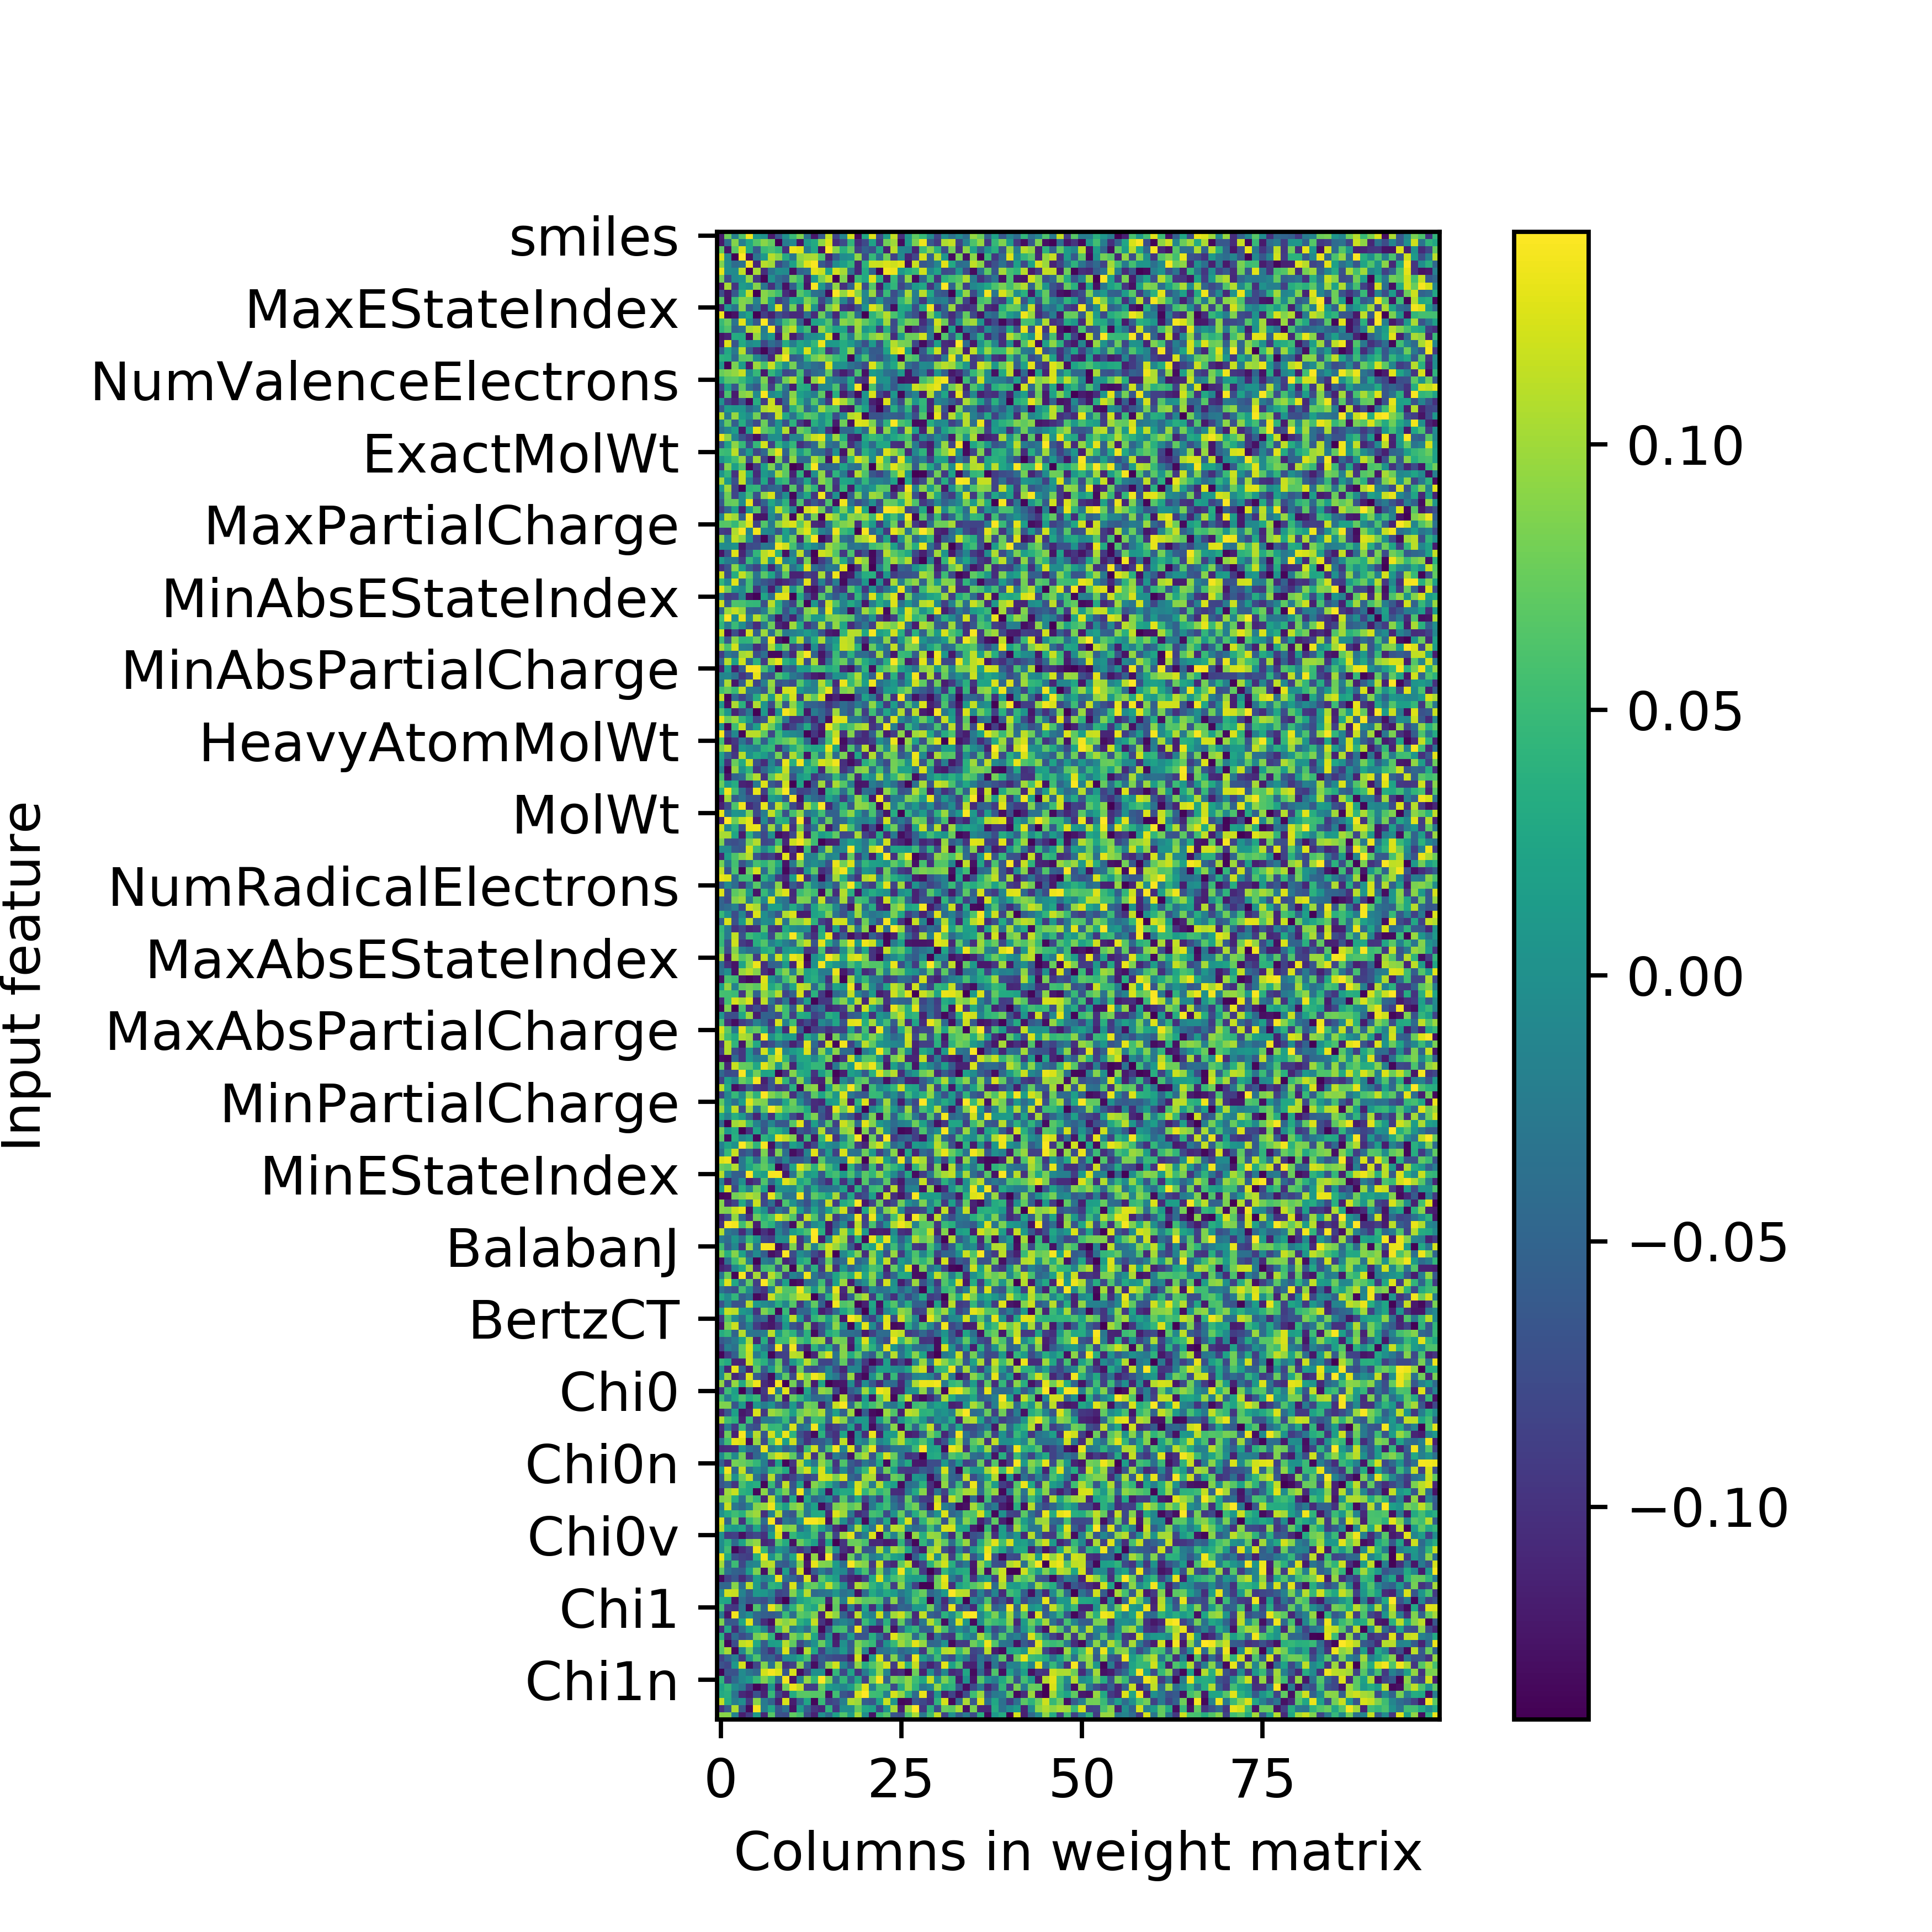
\includegraphics[width=0.8\textwidth,scale=1,totalheight=0.5\textheight]{images/neural_network_activation}
					\caption{Heat map showing the weights learnt in the first layer of the neural network}
					\label{fig:neural_net_activation}
				\end{figure}
				
				\begin{mdframed}[]
					\paragraph{The Learning Algorithm \cite{StephenM2014}}
					\begin{itemize}
						\item \textbf{Initialisation}
						\\ $n$ small (positive and negative) random numbers are assigned as weights $w_{ij}$ where $i$ is the number of weights and $j$ represents the neuron being examined.
						\item \textbf{Training} for T iterations or until all the outputs are correct
						\begin{itemize}
							\item[-] For each input vector $X = [x_1,x_2,x_3,...,x_n]$
							\begin{itemize}
								\item[*] Compute the activation value ($h$) of each neuron $j$: \\
								\begin{equation}
								h = \sum_{i=0}^{n}w_{ij}x_i
								\end{equation}
								\item[*] Calculate the activation ($y$) of neuron $j$ using the activation function $g$: \\
								\begin{equation}
								y_j = g(h) = 
								\begin{cases}
								1 & \text{if h} \textgreater \theta \\
								0 & \text{if h} \le \theta
								\end{cases}
								\end{equation}
								\item[*] Update the weights of neuron $j$ using the formula: \\
								\begin{eqnarray}
								\Delta w_{ij} = - \eta(y_j - t_j) * x_i & \\
								w_{ij} = \Delta w_ij + w_ij
								\end{eqnarray}
								
							\end{itemize}
						\end{itemize}
						\item \textbf{Recall or Prediction}	
						\\To predict the value of new molecule with feature vector $X$ using:
						\begin{equation}
						y_j = g(\sum_{i=0}^{m}w_{ij}x_i) = 
						\begin{cases}
						1 & \text{if } w_{ij}x_i \textgreater 0 \\
						0 & \text{if } w_{ij}x_i \le 0
						\end{cases}
						\end{equation}
						where 1 represents a molecule that passes through the barrier and 0 a molecule that doesn't.
					\end{itemize}
				\end{mdframed}
			%\paragraph{Model Training}
			%For both datasets (simple molecular descriptors and fingerprint), they were rescaled to have a minimum of -1 and a Maximum of 1. The transformed data was then trained on a neural network and an accuracy of $\sim86\%$ was achieved. \\
			\paragraph{Optimisations for Model Training} 
			\underline{Univariate Model Selection}: \\
			Here for each input data point in the feature vector, we compute whether there is a statistical relationship between the input and the target. The input features which are calculated to be highly unrelated to the target are then dropped from the dataset. Applying this model selection to the molecular descriptor dataset with a percentile of 50 gives us the features in figure \ref{fig:neuralnetworksmdunivariate}.
				\begin{figure}[h]
					\centering
					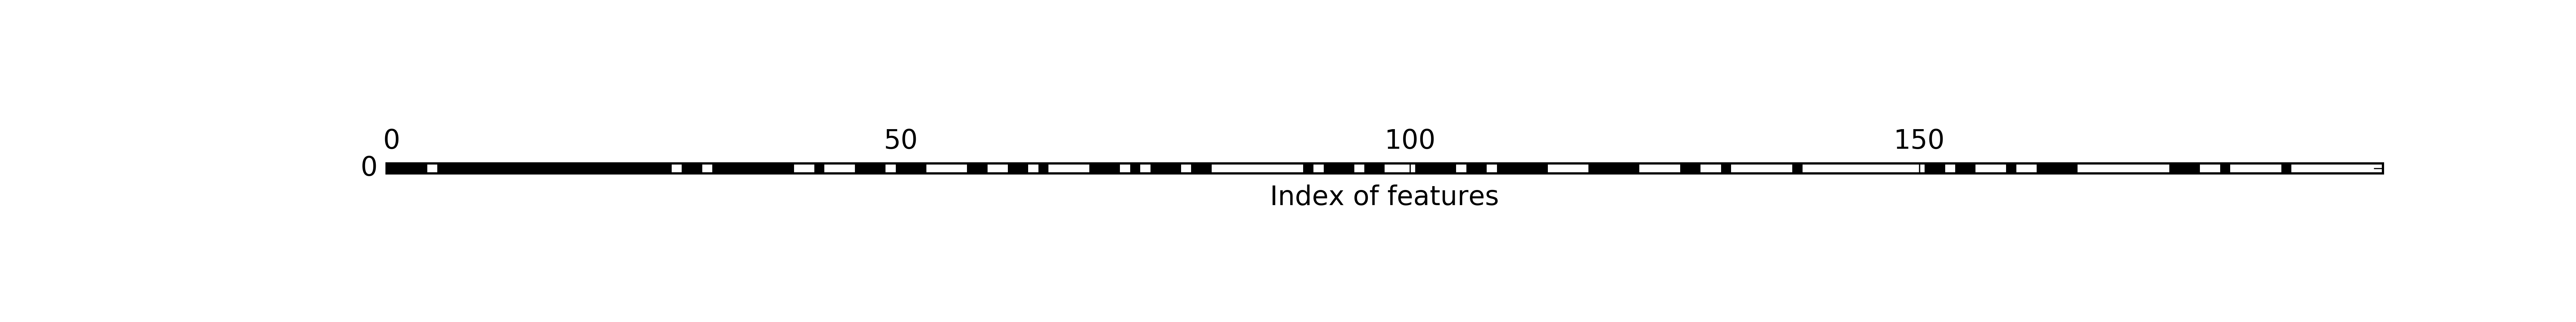
\includegraphics[width=\textwidth,scale=1]{images/neural_network_smd_univariate_matrix}
					\caption{Matrix diagram of selected features}
					\label{fig:neuralnetworksmdunivariate}
				\end{figure}
			The neural network was then trained with the new feature vector and a percentage increase in accuracy was achieved - with a new accuracy of $\sim87\%$ on the molecular descriptor dataset and an accuracy of $\sim88\%$ on the fingerprint dataset.
			
			
			
		\subsection{Ensemble Classifiers} \label{subsection:ensemble}
		Ensembles were used earlier to combine many decision trees to achieve better classification results. 
		
		Ensembles have the benefit that they tend to perform better than single classifiers \cite{Dietterich}; With this knowledge, all the previously trained classifier were combined to create an ensemble learner that makes predictions by taking a weighted vote of the individual prediction of the classifiers its composed of.
		
		The ensemble classifier achieved an accuracy of $\sim94\%$ on both the simple molecular and the fingerprint dataset; Which further enforces the claim by Thomas G. Dietterich \cite{Dietterich} that ensemble learners perform better than individual learners.
		
		

\chapter{Model Evaluation and Persistence(Notes)}
	\section{Model Evaluation}
		% Draw a diagram like the one in this link(http://machinelearningmastery.com/compare-machine-learning-algorithms-python-scikit-learn/) to compare the results of all the classifiers
		%TODO: Talk about Cross validation, include diagrams like in scikit-learn pg 252, the entire chapter is a valuable resource	
				
		\subsection{Classifier Performance Comparison}
		\begin{table}[ht]
			\caption{Classifier average performance on different datasets}
			\centering
			\begin{tabular}{c|c|c}	
				\hline\hline
				Classifier & Simple Molecular descriptors(\%) & Morgan Fingerprint(\%) \\
				\hline
				Decision Tree & 80 & 79 \\
				Extra Trees & 86 & 84 \\
				Random Forests & 85 & 84 \\
				AdaBoost Decision Trees & 84 & 82 \\
				Gradient Boosted Trees & 86 & 82 \\
				k-Nearest Neighbours & 87 & 89 \\ 
				Support Vector Machines & 84.9 & 84.9 \\
				Neural Networks & 87 & 88 \\
				\hline
			\end{tabular}
		\end{table}
	%\section{Model Improvement techniques}
		%\subsection{Grid Search}
	\section{Model Persistence} 
	%How you will use pickle to persist the model
		
		


\chapter{Conclusion}
	\section{Integration into a Web Application}
	
	\section{Deployment}
	\section{Areas for improvement}



\chapter*{Appendix}
\begin{figure}[H]
	\centering
	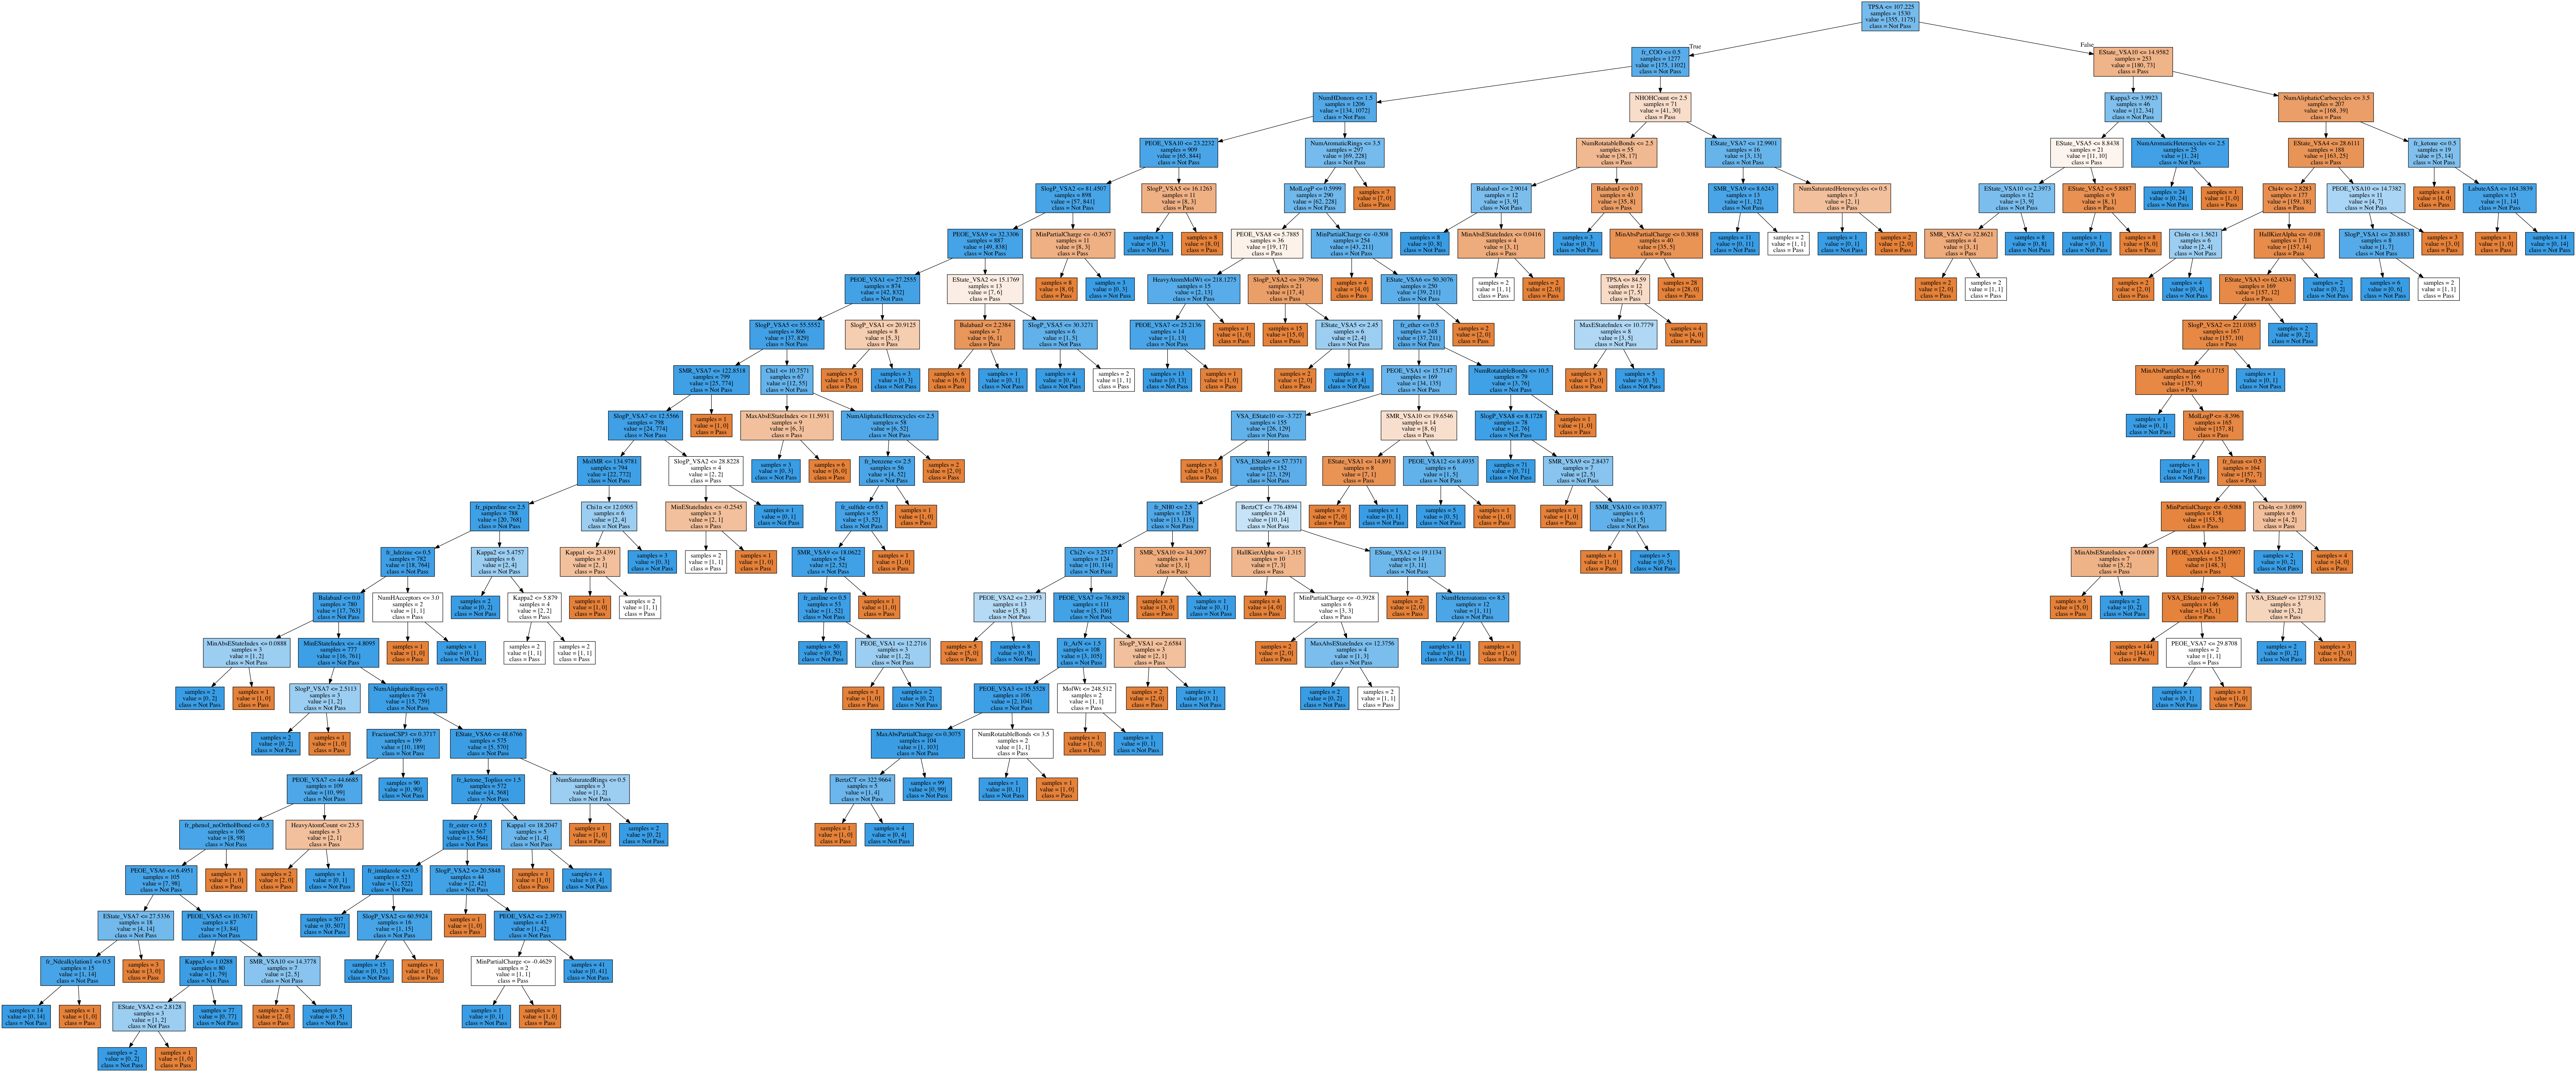
\includegraphics[width=\textwidth,scale=1,height=\textheight]{images/bbb_tree_smd}
	\caption{Decision Tree: Simple Molecular Descriptors}
	\label{fig:bbb_tree_smd_large}
\end{figure}


\bibliographystyle{plain}
\bibliography{ibraheem_aj_dissertation}

\end{document}